% !TeX root = RJwrapper.tex
\title{animbook: Visualizing changes in performance measures and demographic affiliations using animation}
\author{by Krisanat Anukarnsakulchularp}

\maketitle

\abstract{%
Categorical data has often been presented statically despite its potential to unveil an intriguing movement pattern relevant to the various domains of data, including company ranking quantile in the accounting data and shifts in voter party affiliations. Inspired by the animation in the New York Times article ``Extensive data show punishing reach of racism for black boys,'' this paper aims to develop an R package, animbook, that can generalize the animation to suitably apply to a wider range of data. The package included a function that allowed for the transformation of the data and connection with elements of the plot that would be animated. This results in an animation tool that helps communicate complex data, enhancing the narrative and keeping it engaged for the general audience.
}

\hypertarget{intro}{%
\section{Introduction}\label{intro}}

The concept of ``zombie companies'' began to attract attention when Caballero, Hoshi, and Kashyap (2008) reported on their proliferation in Japan. Zombie companies are those with an interest coverage ratio of less than one for a period of more than three years, that is, companies taking space in the market but adding no life to the economy. We would detect their presence by a drop in performance, which is a movement pattern in their relative ranking over time. Generally, studying movement patterns is interesting for many problems, including rocket ship startups that rapidly perform well, or in politics, to study voters who switch party affiliation between elections. Viewing changes between categories over time is an interesting challenge for visualization.

The New York Times provided a possible solution in the article titled ``Extensive data show punishing reach of racism for black boys'' (Badger et al. (2018)) to tell the story of how racism appears to inhibit socioeconomic change. This animation is the motivation for the new visualization presented here, to be applied generally.

The challenge in producing an animation like that in New York Times article animation is the transformation of the data, and connection with elements of the plot that will be animated. The complexities include standardizing starting times of the temporal variable, allowing for the user to choose the number of categories, standardizing distributions and allowing the user to input pre-computed categorical data. These considerations provide the objective for creating an R package that can generalize the animation to suitably apply to a wide range of data.

The structure of this paper is as follows. The next section explains the animation in The New York Times article and why it is relevant to the problem of studying zombie companies. The next section describes the expected data format. Following this is an explanation of available animation tools, and how they are employed for this problem. A section on the functions of the package and how the visualization is designed, demonstrates how the data is mapped to the animation. The last two sections illustrate the usage of the package and applications to company performance and changing political allegiance.

\hypertarget{NYTvis}{%
\section{Explanation of the New York Times visualization}\label{NYTvis}}

\begin{figure}

{\centering 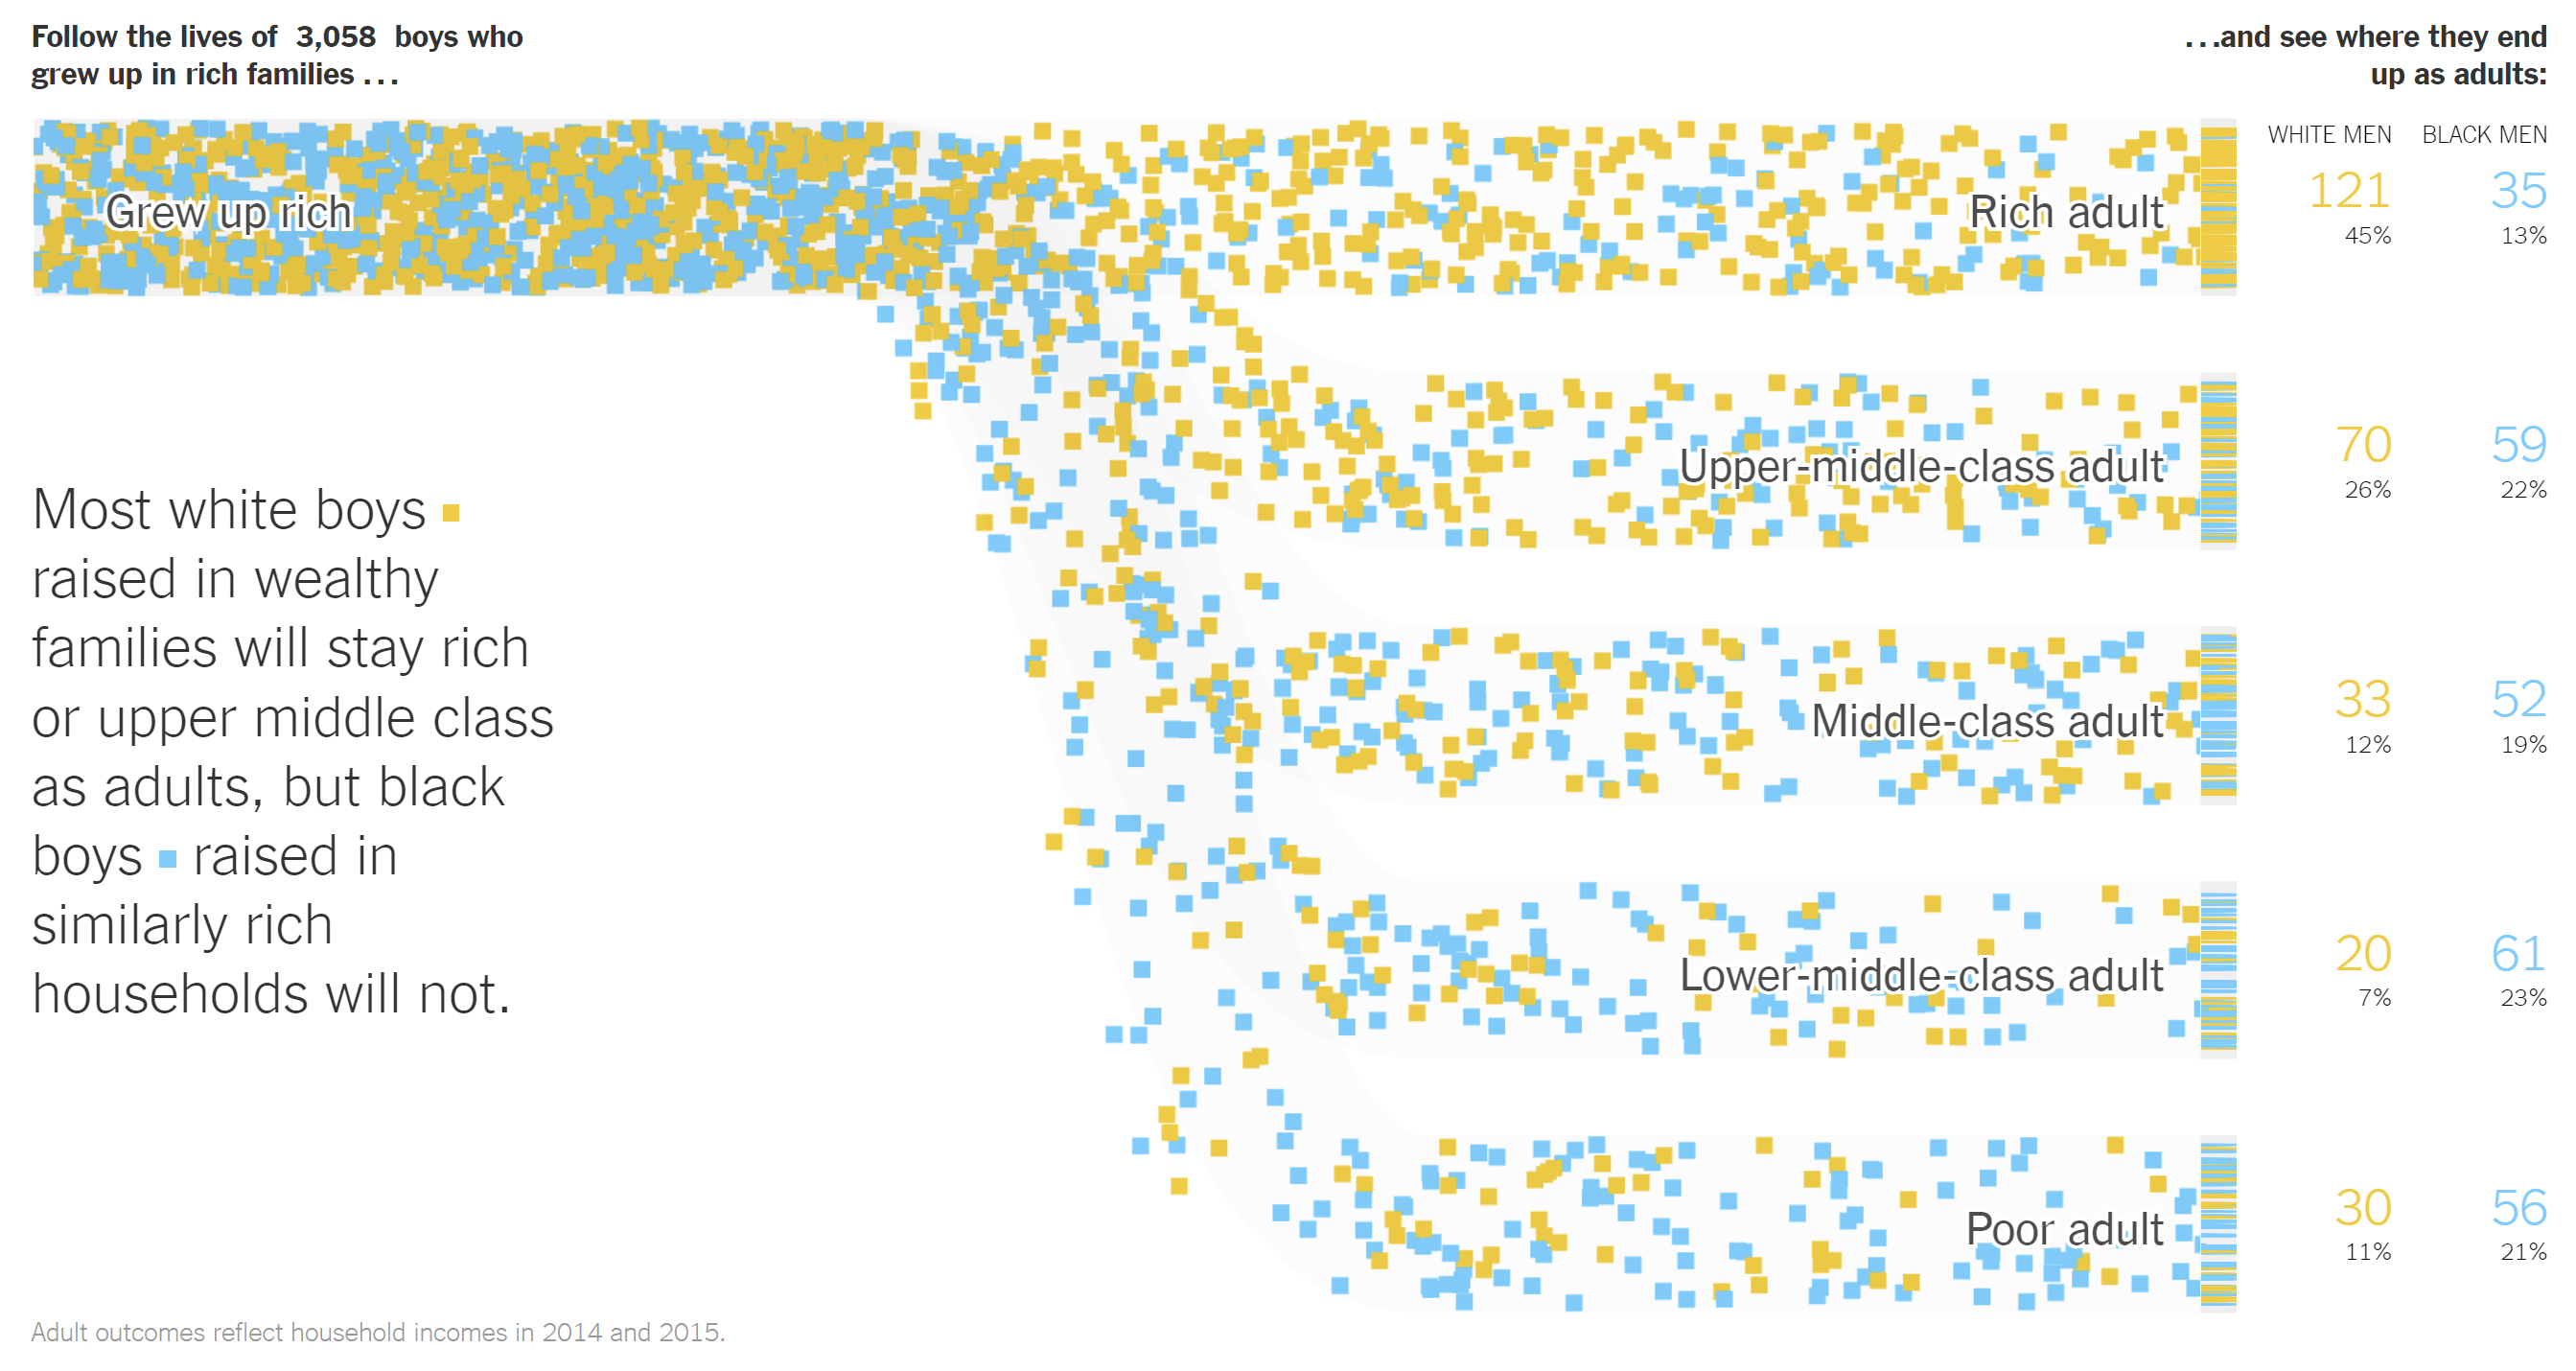
\includegraphics[width=1\linewidth]{figures/NYT} 

}

\caption{Screenshot of the New York Times animation, which is the motivation for this visualization package..}\label{fig:nyt}
\end{figure}

The interactive chart featured in the New York Times article (Figure \ref{fig:nyt}) unveils the issue of income disparities between black and white children who were raised in families with comparable income according to the Chetty et al. (2020). This visualization reveals that, compared to white children, black children are more likely to drop down to the lower-income group, given that they both grew up in wealthy families.

In the visualization, each observation is initially classified into one group at the start and potentially transitions into either the same group or a different group. This dynamics visualization constructs questions on the broader use of this visualization to other types of data. The potential use of this visualization on accounting data is to convey a message, as reported by the McGowan, Andrews, and Millot (2017), that the concept of zombie companies is not unique to Japan alone. It is also present in the United States, which has a faster metabolize rate (more new listings and exits) relative to Japan.

The political data that exhibits the movement of voters switching party affiliations between elections can be a valuable insight into the behavior of the voters. This data could be extended to incorporate demographic information about the voters, providing analysts with a significant insight into voter behavior. This allows them to consolidate effective campaigns for their political party. This also applies to marketing data, where customers shift their product interest to the competitor, providing the marketing analysts with an understanding of both the company's products and the overall market.

This animation was developed using two software based on JavaScript, D3.js (Bostock (2012)), and WebGL (reference). The D3 JavaScript is one of the most widely known libraries for creating an interactive and dynamic visualization. It enables the designers to bind both the data and graphical elements to the DOM (Document Object Model). On the other hand, WebGL functions as a JavaScript API for rendering interactive 2D and 3D graphics within any compatible web browser without the use of plug-ins. For the animation in this paper, the programming language that will be used for recreating and revising the visualization done by The New York Times articles is R (R Core Team (2021)).

\hypertarget{data}{%
\section{Data}\label{data}}

\begin{figure}

{\centering 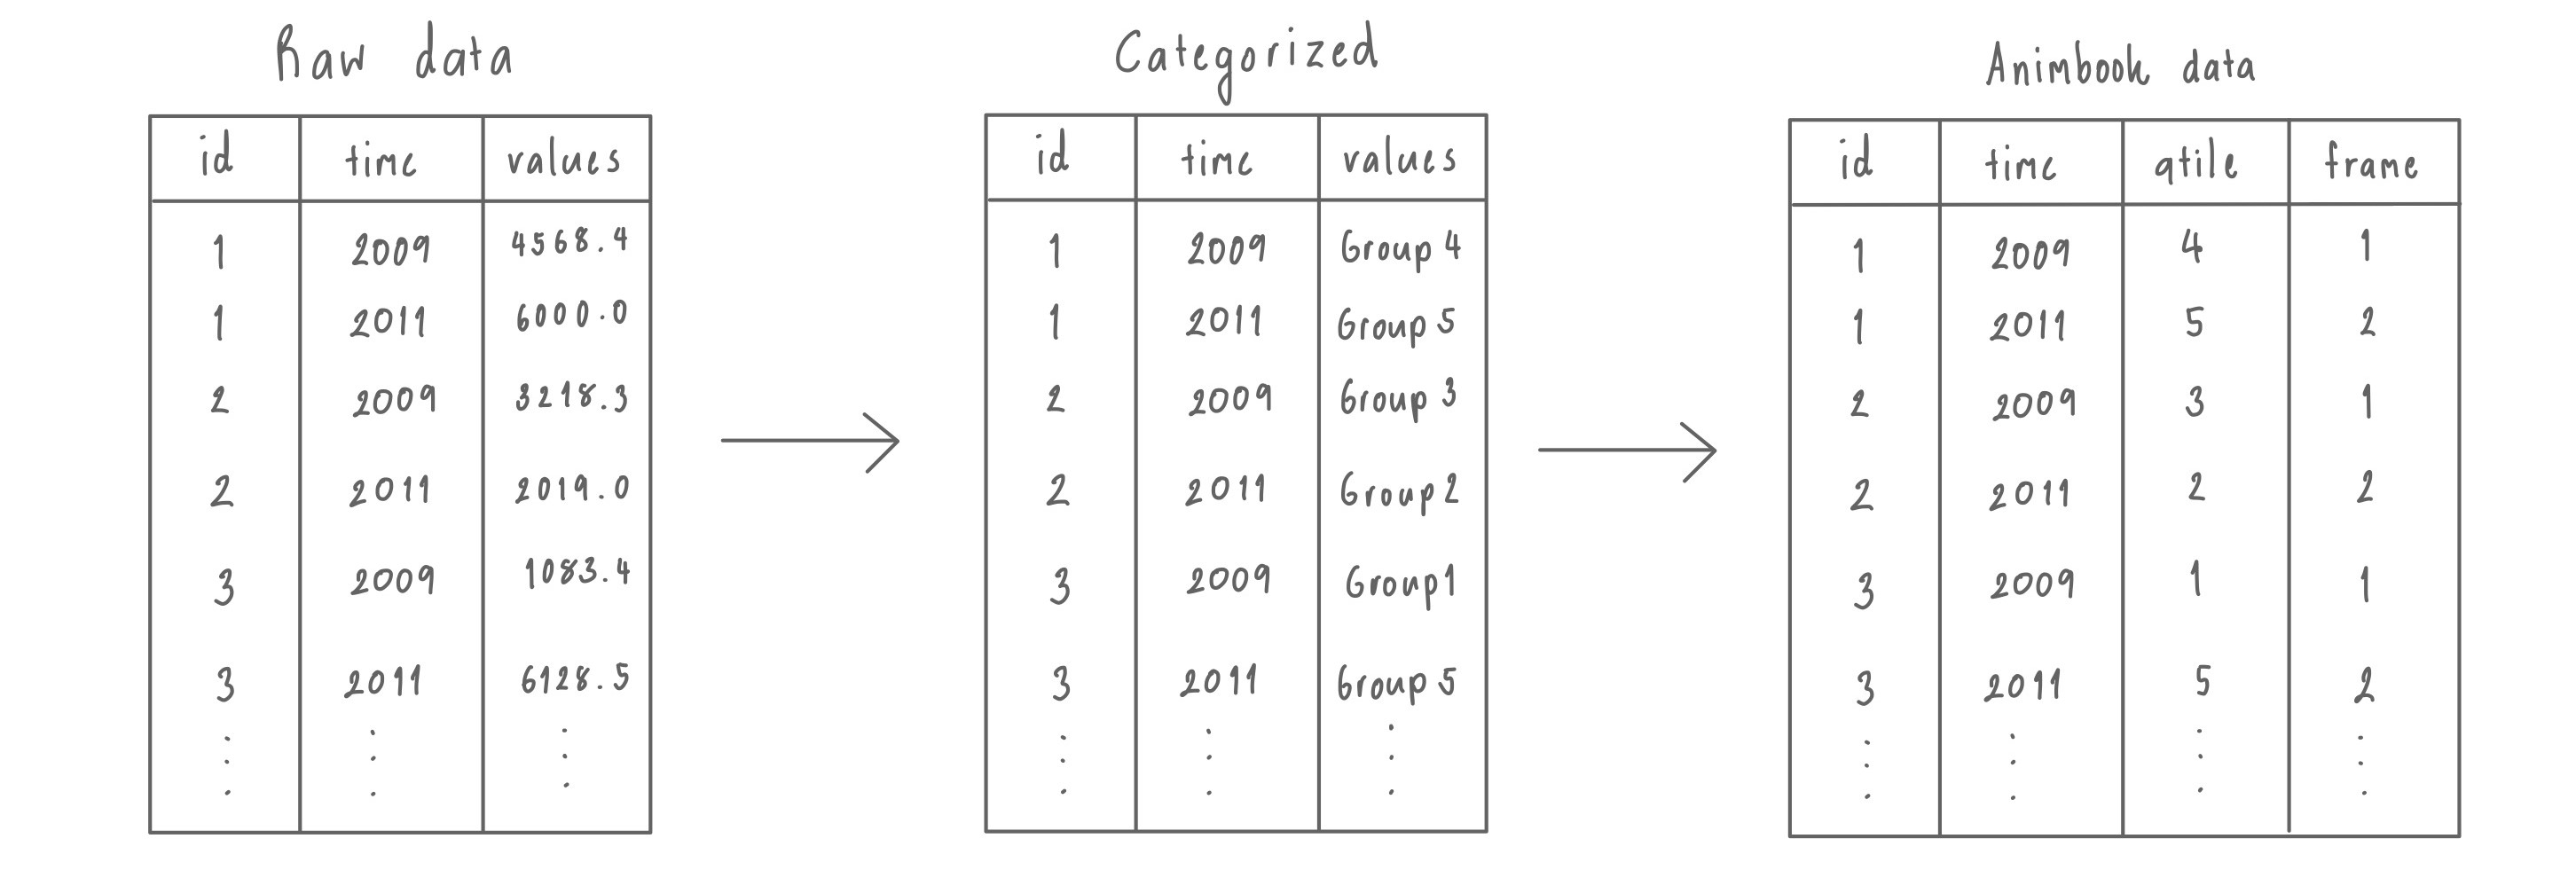
\includegraphics[width=1\linewidth]{figures/data-diagram} 

}

\caption{The animation expects data with an ID and a time variable, along with a numerical variable (raw form), which is possibly converted to categorical (categorized). The data can be provided in the raw or categorized form and will be processed into the format needed for the animation, where the categorical variable is treated as a quantile and an animation frame variable is created.}\label{fig:data-diagram}
\end{figure}

In the data structure, there are requirements that must be followed for reproducing the animation. First, the data set needs to be in the \texttt{tidy\ data} format (Wickham (2014)). The data then must have at least ID and time variables, in addition to the measured variables, which would usually be numeric but can also be categorical as well. The ID variable indicates the individual, which is followed over time, such as the company name. There may also be a grouping variable, such as the country where the company is registered.

Figure \ref{fig:data-diagram} illustrates the expected format of the data and variables created to prepare it for the animation. We start with the raw data structure. The values are presented in the numerical format, which we call the `raw' form. In most cases, the measured variable will be numerical and require transformation. The second form is categorized data, which involves transforming numerical variables into categories, typically quantiles. This transformation may not be necessary if it is already provided in the categorized format. The last form is animated data, where the frame is assigned to each unique ID.

\hypertarget{animation}{%
\section{Animation tools}\label{animation}}

\begin{figure}

{\centering 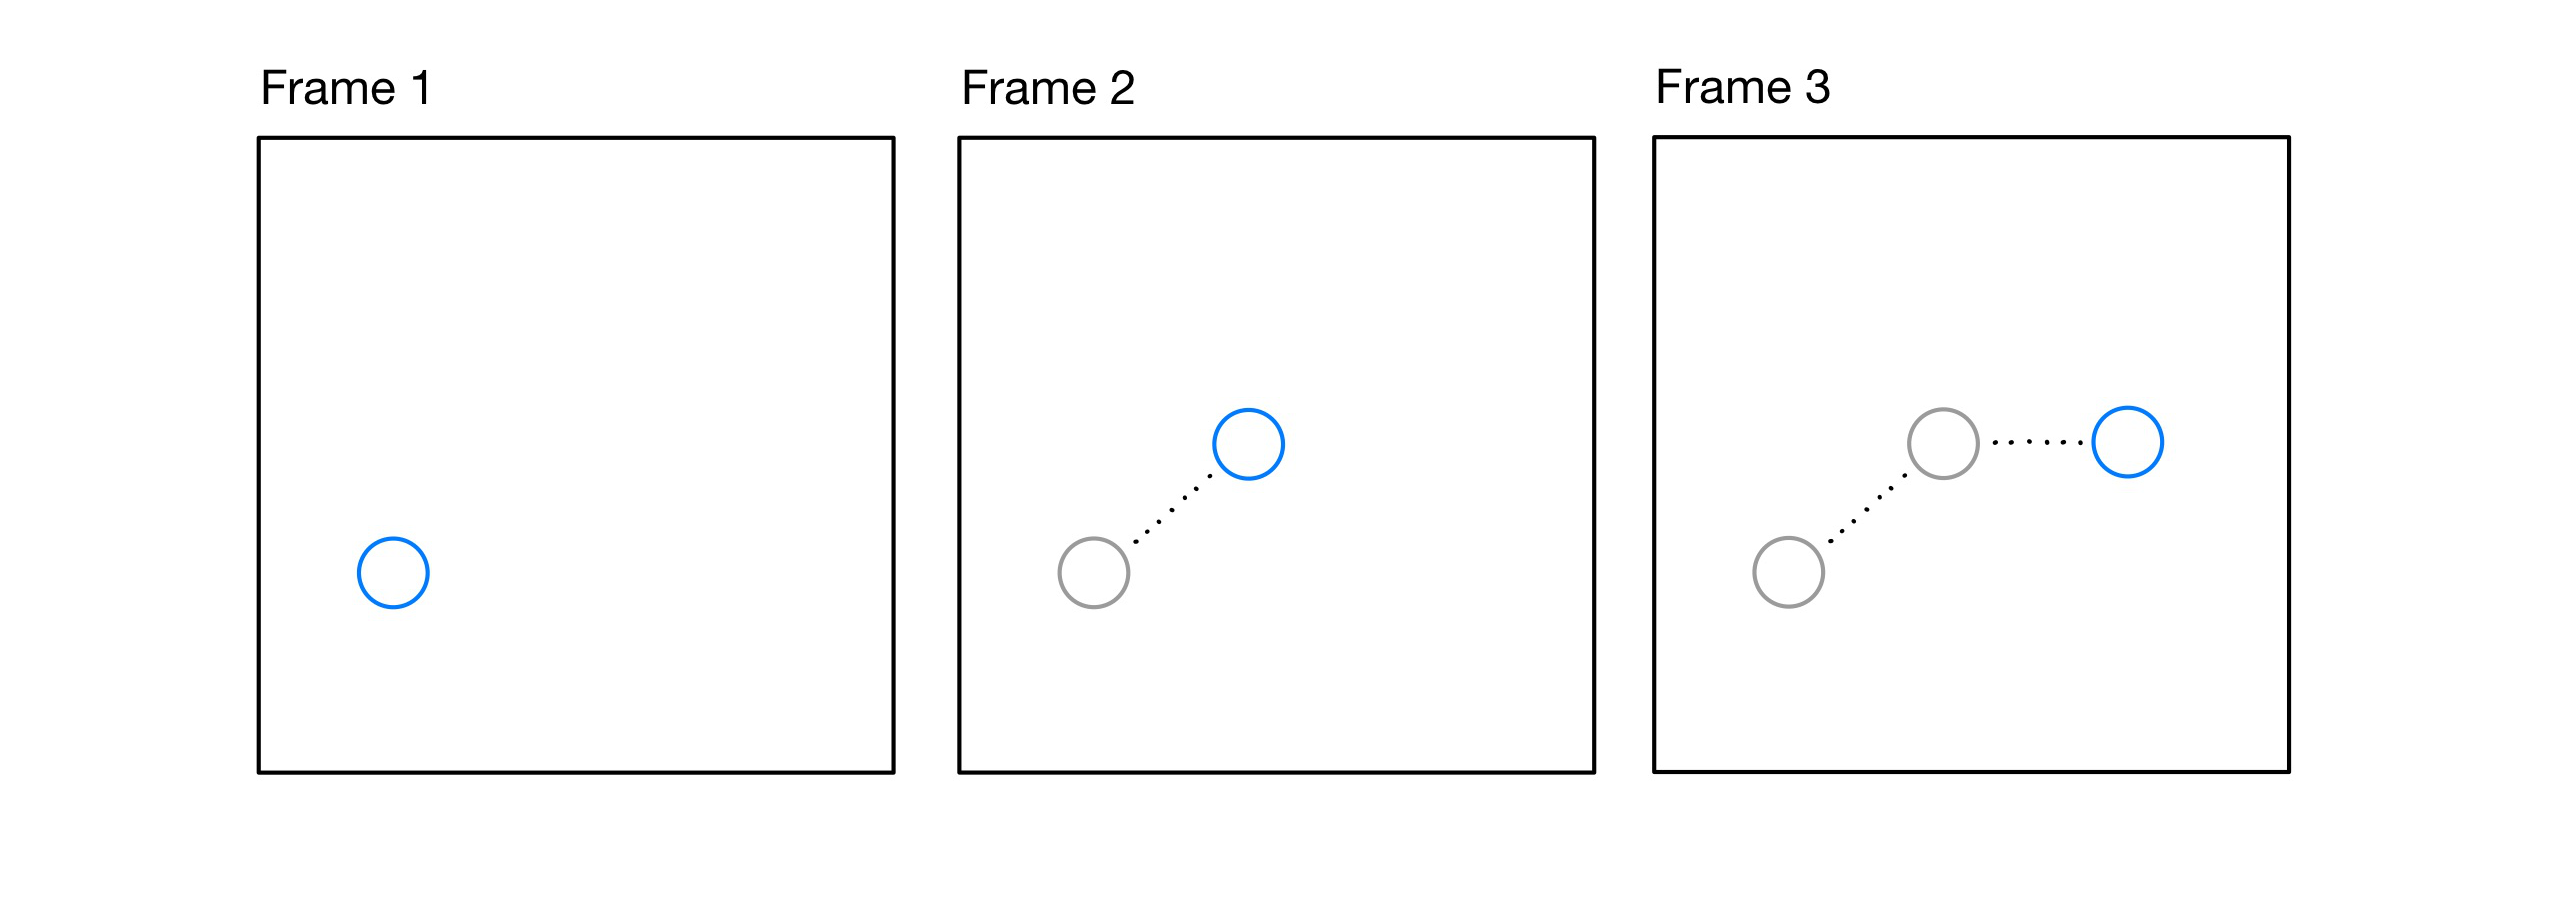
\includegraphics[width=1\linewidth]{figures/animation-diagram} 

}

\caption{The diagram shows how the animation is done using the successive pictures. When small changes are seen in quick succession, it will appear as if the objects are in motion.}\label{fig:animation-diagram}
\end{figure}

A principle important for designing a useful animation is called persistence of vision (Webster (2005)). When an image disappears, the brain will retain the previous images for a brief period of time. It is this slight period of retention that allows humans to separate sequential images. If this is seen in quick succession, it will appear as if the objects are in motion. This is illustrated in Figure \ref{fig:animation-diagram}.

There are multiple ways to create an animation in the R environment (R Core Team (2021)), including the packages \CRANpkg{gganimate} (Pedersen and Robinson (2020)) and \CRANpkg{plotly} (Sievert (2020)).

The \CRANpkg{gganimate} package is an extension from the \CRANpkg{ggplot2} package (Wickham (2016)) to include the description of an animation. It added new grammar classes to the plot object, allowing it to understand how the plot should change over time. The use of \texttt{transition\_*()} functions allows it to achieve this by specifying how the data evolves and how it relates to itself across time. This includes \texttt{gifski\_renderer()} from the \CRANpkg{gifski} package \{Ooms (2023b)\} to save animation in GIF format or \texttt{av\_renderer()} from the \CRANpkg{av} package \{Ooms (2023a)\} to save it into a video file format.

The \texttt{plotly} software is a graphic library that provides tools for creating an interactive plot in multiple programming languages, such as R, JavaScript, Python, and Julia. In R, plotly can be accessed through the \CRANpkg{plotly} package, which integrates plotly.js from the JavaScript graphing library. The usage of this library can be from a converting function, \texttt{ggplotly()}, or a standalone function, \texttt{plot\_ly()}. The conversion is accomplished by taking the elements from the \texttt{ggplot} object and then redrawing them using the plotly.js.

\begin{figure}

{\centering 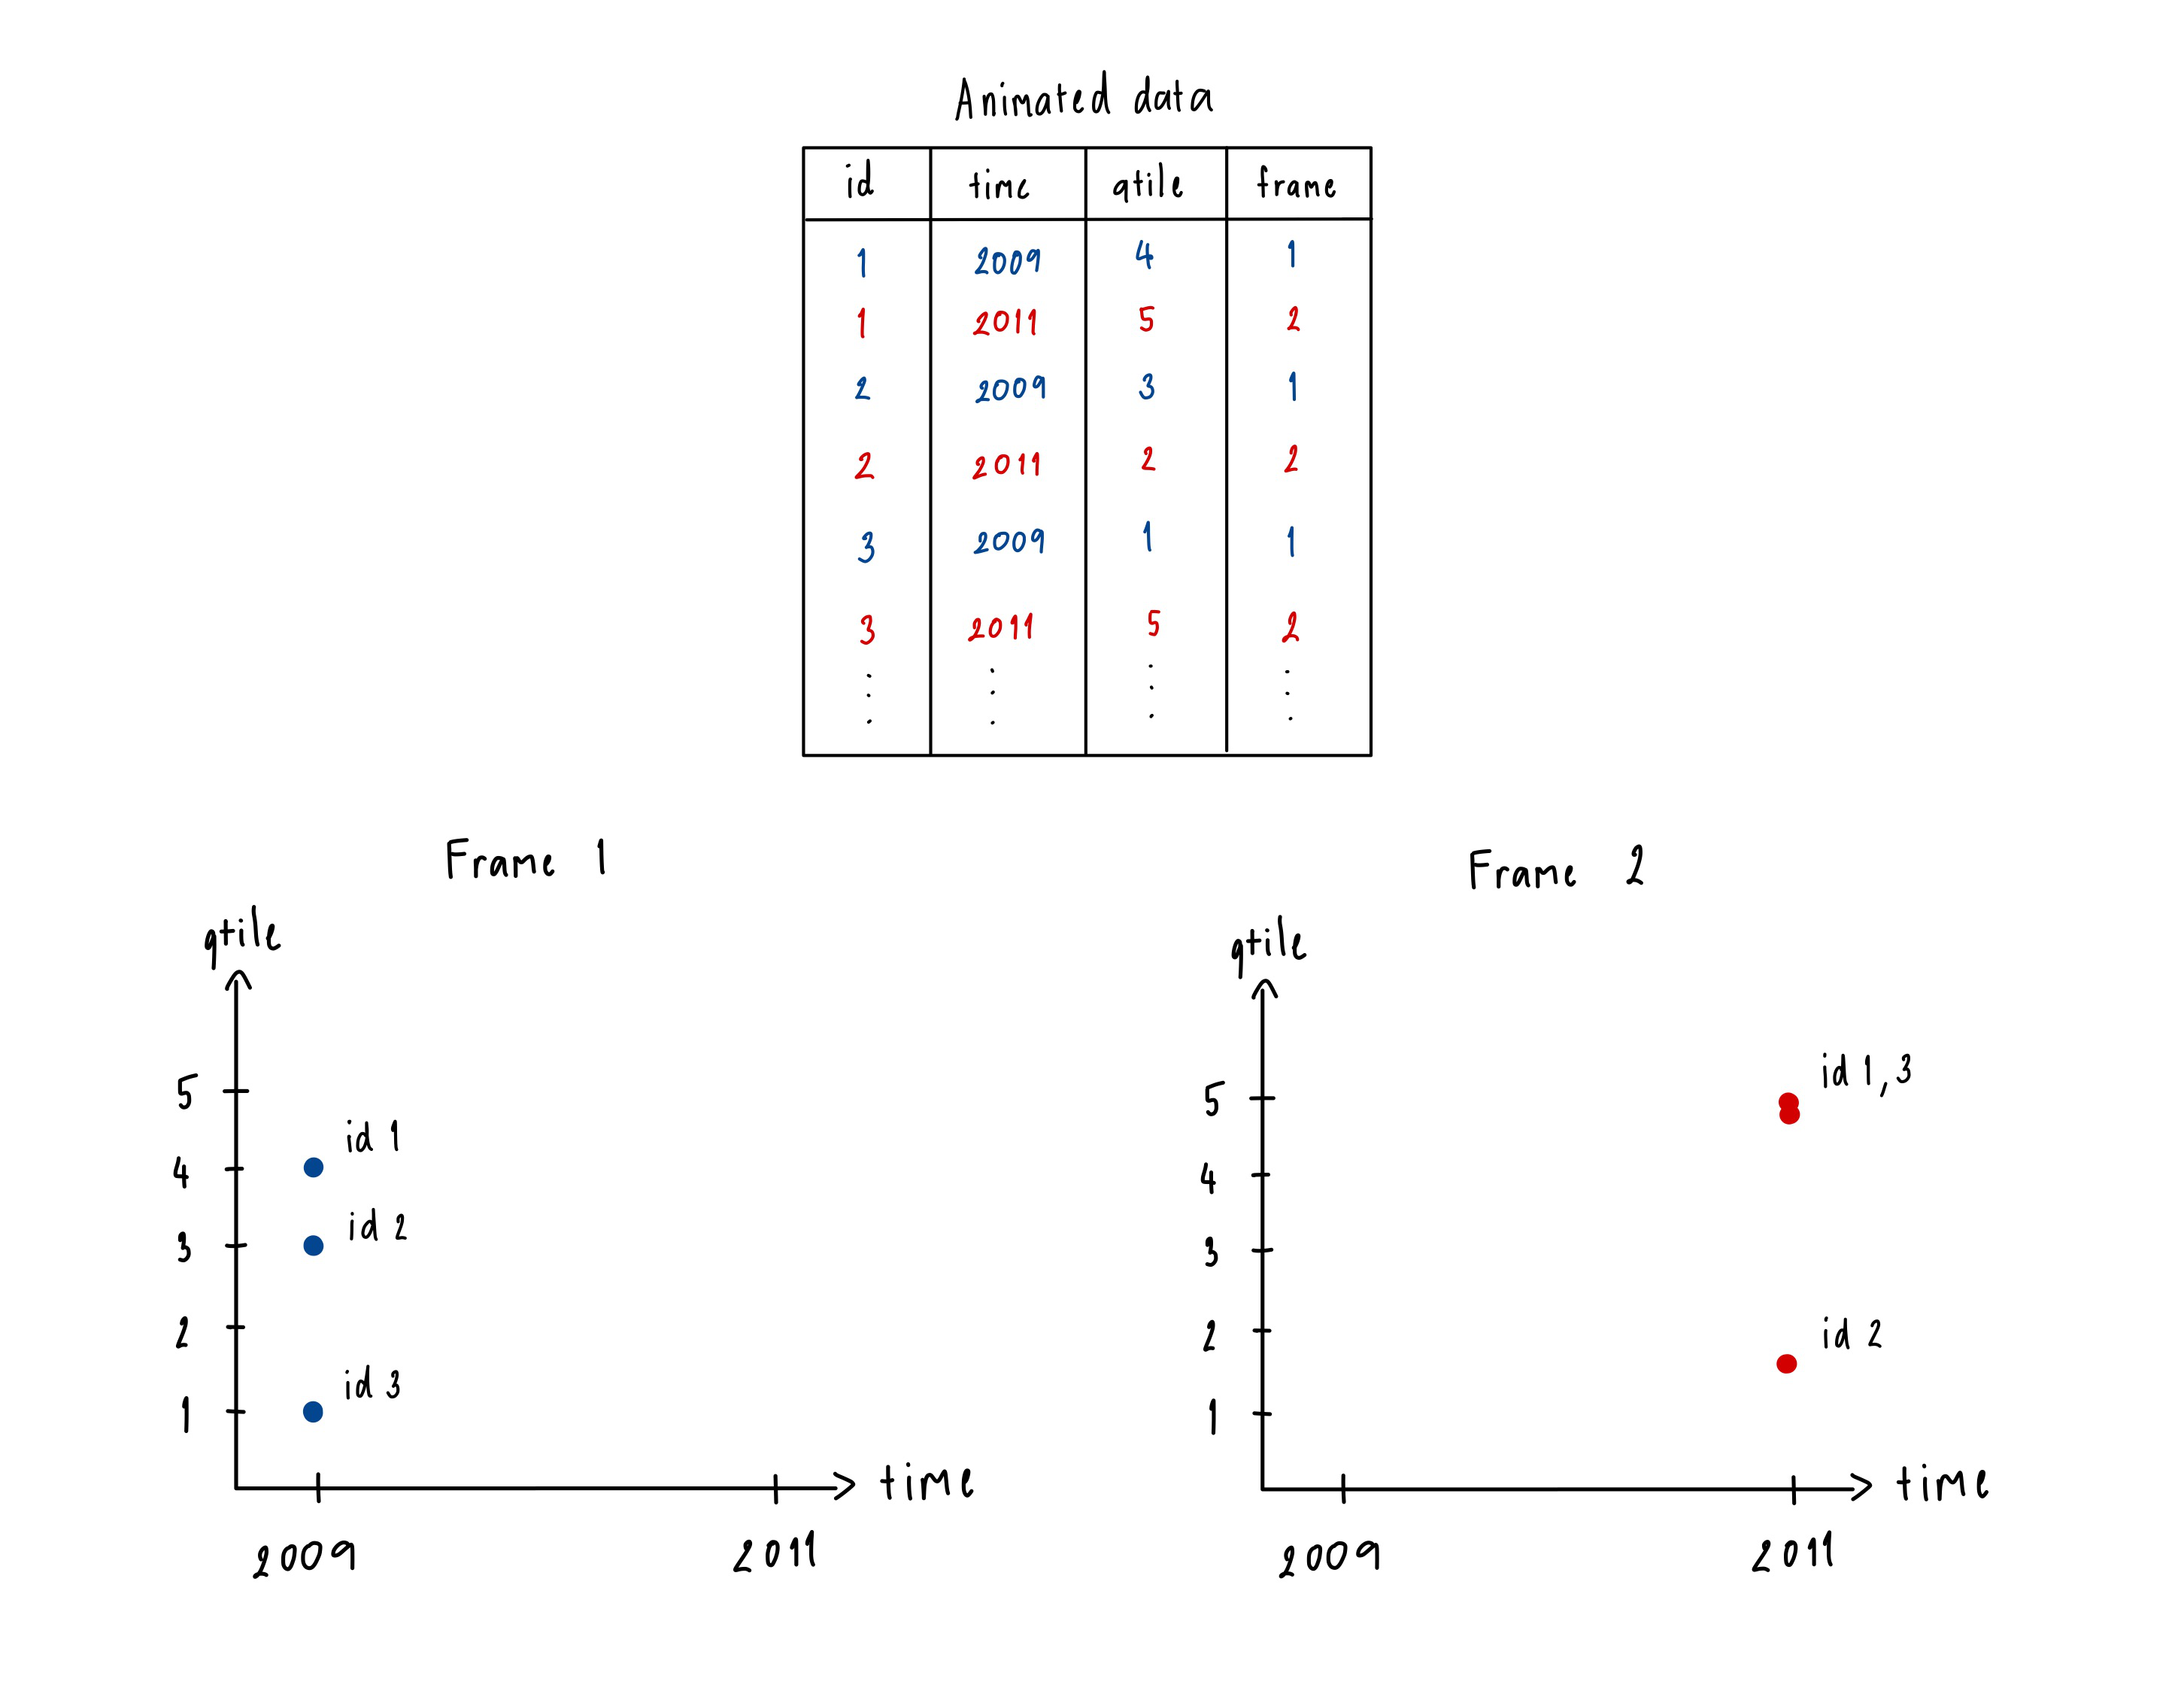
\includegraphics[width=1\linewidth]{figures/animated-diagram} 

}

\caption{The diagram shows how the frames were used in the animated plot. Frame one is depicted in blue, and frame two is represented in red. Each blue component is mapped exclusively to the Frame 1 plot, while all the second-frame elements are excluded, and vice versa.}\label{fig:animated-diagram}
\end{figure}

In the context of data, as shown in Figure \ref{fig:animated-diagram}, observations are positioned at specific points in time. The further the distance between these points, the less smooth the animation becomes. This issue can be eliminated by interpolating additional points in between the observations. In the \CRANpkg{gganimate} package, the interpolation is achieved using the \CRANpkg{tweenr} package (Pedersen (2022)), while in \CRANpkg{plotly}, it utilizes d3.interpolate (Bostock (2012)).

Figure \ref{fig:animated-diagram} demonstrates how the frame variables are applied in an animated plot. The frame variable within the animated data structure allows the animation function to determine the position of observations on the plot at any given frame.

From Hasler, Kersten, and Sweller (2007), it suggests that having control options for the animation can improve the efficiency of the learning process. Additionally, the length and speed of the animation should also be taken into consideration. According to R. Mayer (2010), the working memory, responsible for selecting and processing information from sensory memory, only holds a processed version of what was presented for generally less than thirty seconds.

In \CRANpkg{gganimate}, the issue of integrating controls can be addressed by setting the \texttt{renderer} argument to be \texttt{av\_renderer()}, which allows the animation output to be in media applications provided in their systems. As for adjusting the length and speed of the animation, the \texttt{nframes} and \texttt{fps} arguments can be utilized. The \texttt{nframes} dictates the number of frames to be rendered, while \texttt{fps} controls how many frames are displayed in one second. Using these two parameters, the duration of the animation in seconds can be calculated as follows: length = nframes/fps.

In the case of \CRANpkg{plotly}, control integration is already implemented by default. The \texttt{frame} and \texttt{transition} arguments within the \texttt{animation\_opts()} function can be specified to set the length and speed of the animation.

\hypertarget{design}{%
\section{Visualization design}\label{design}}

The animated visualization can be an effective communication tool (R. E. Mayer and Moreno (2002); Robertson et al. (2008)). It helps with communicating complex data, enhancing the narrative, and keeping it engaged for the audience. According to R. E. Mayer and Moreno (2002), animation can improve learning, especially when the goal is to promote deep understanding.

R. E. Mayer (2005) states that designing multimedia requires the designer to understand how people learn. One of the principles in R. E. Mayer (2005), Redundancy, suggests that a piece of excess information could overload the learners. By this principle, the animation must be carefully designed to avoid this pitfall.

\begin{figure}
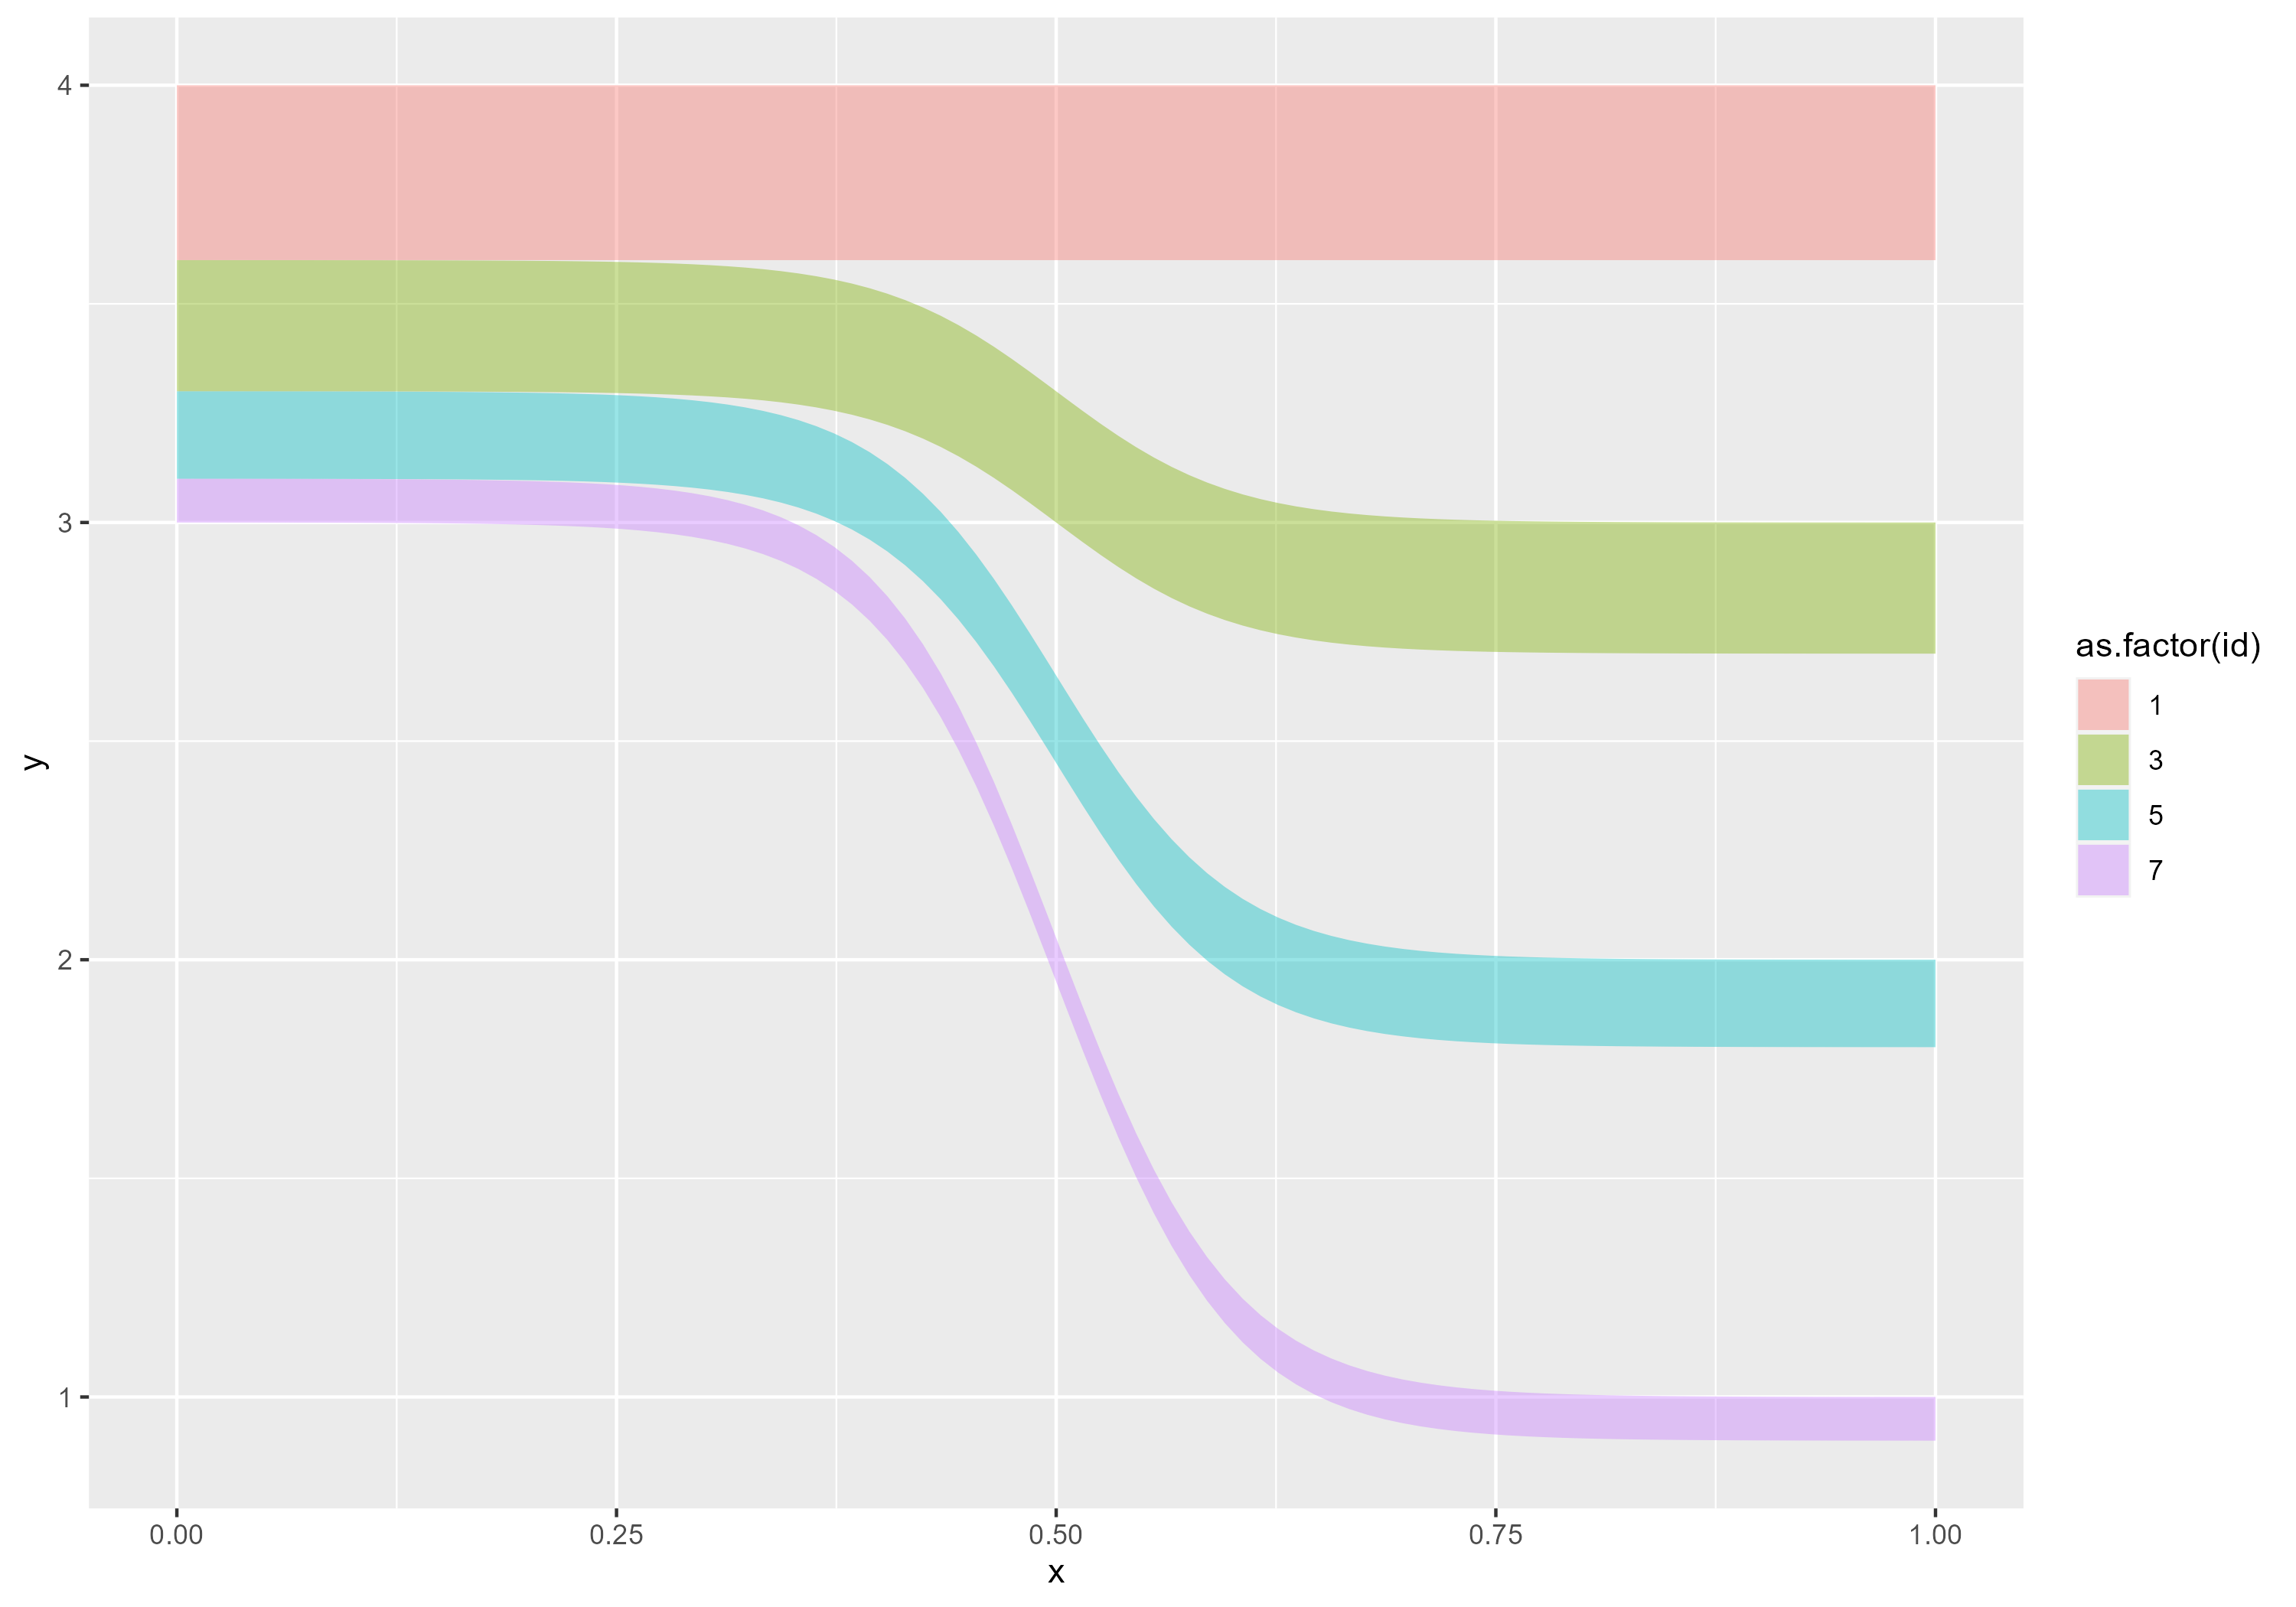
\includegraphics[width=0.5\linewidth]{figures/sigmoid-shade} 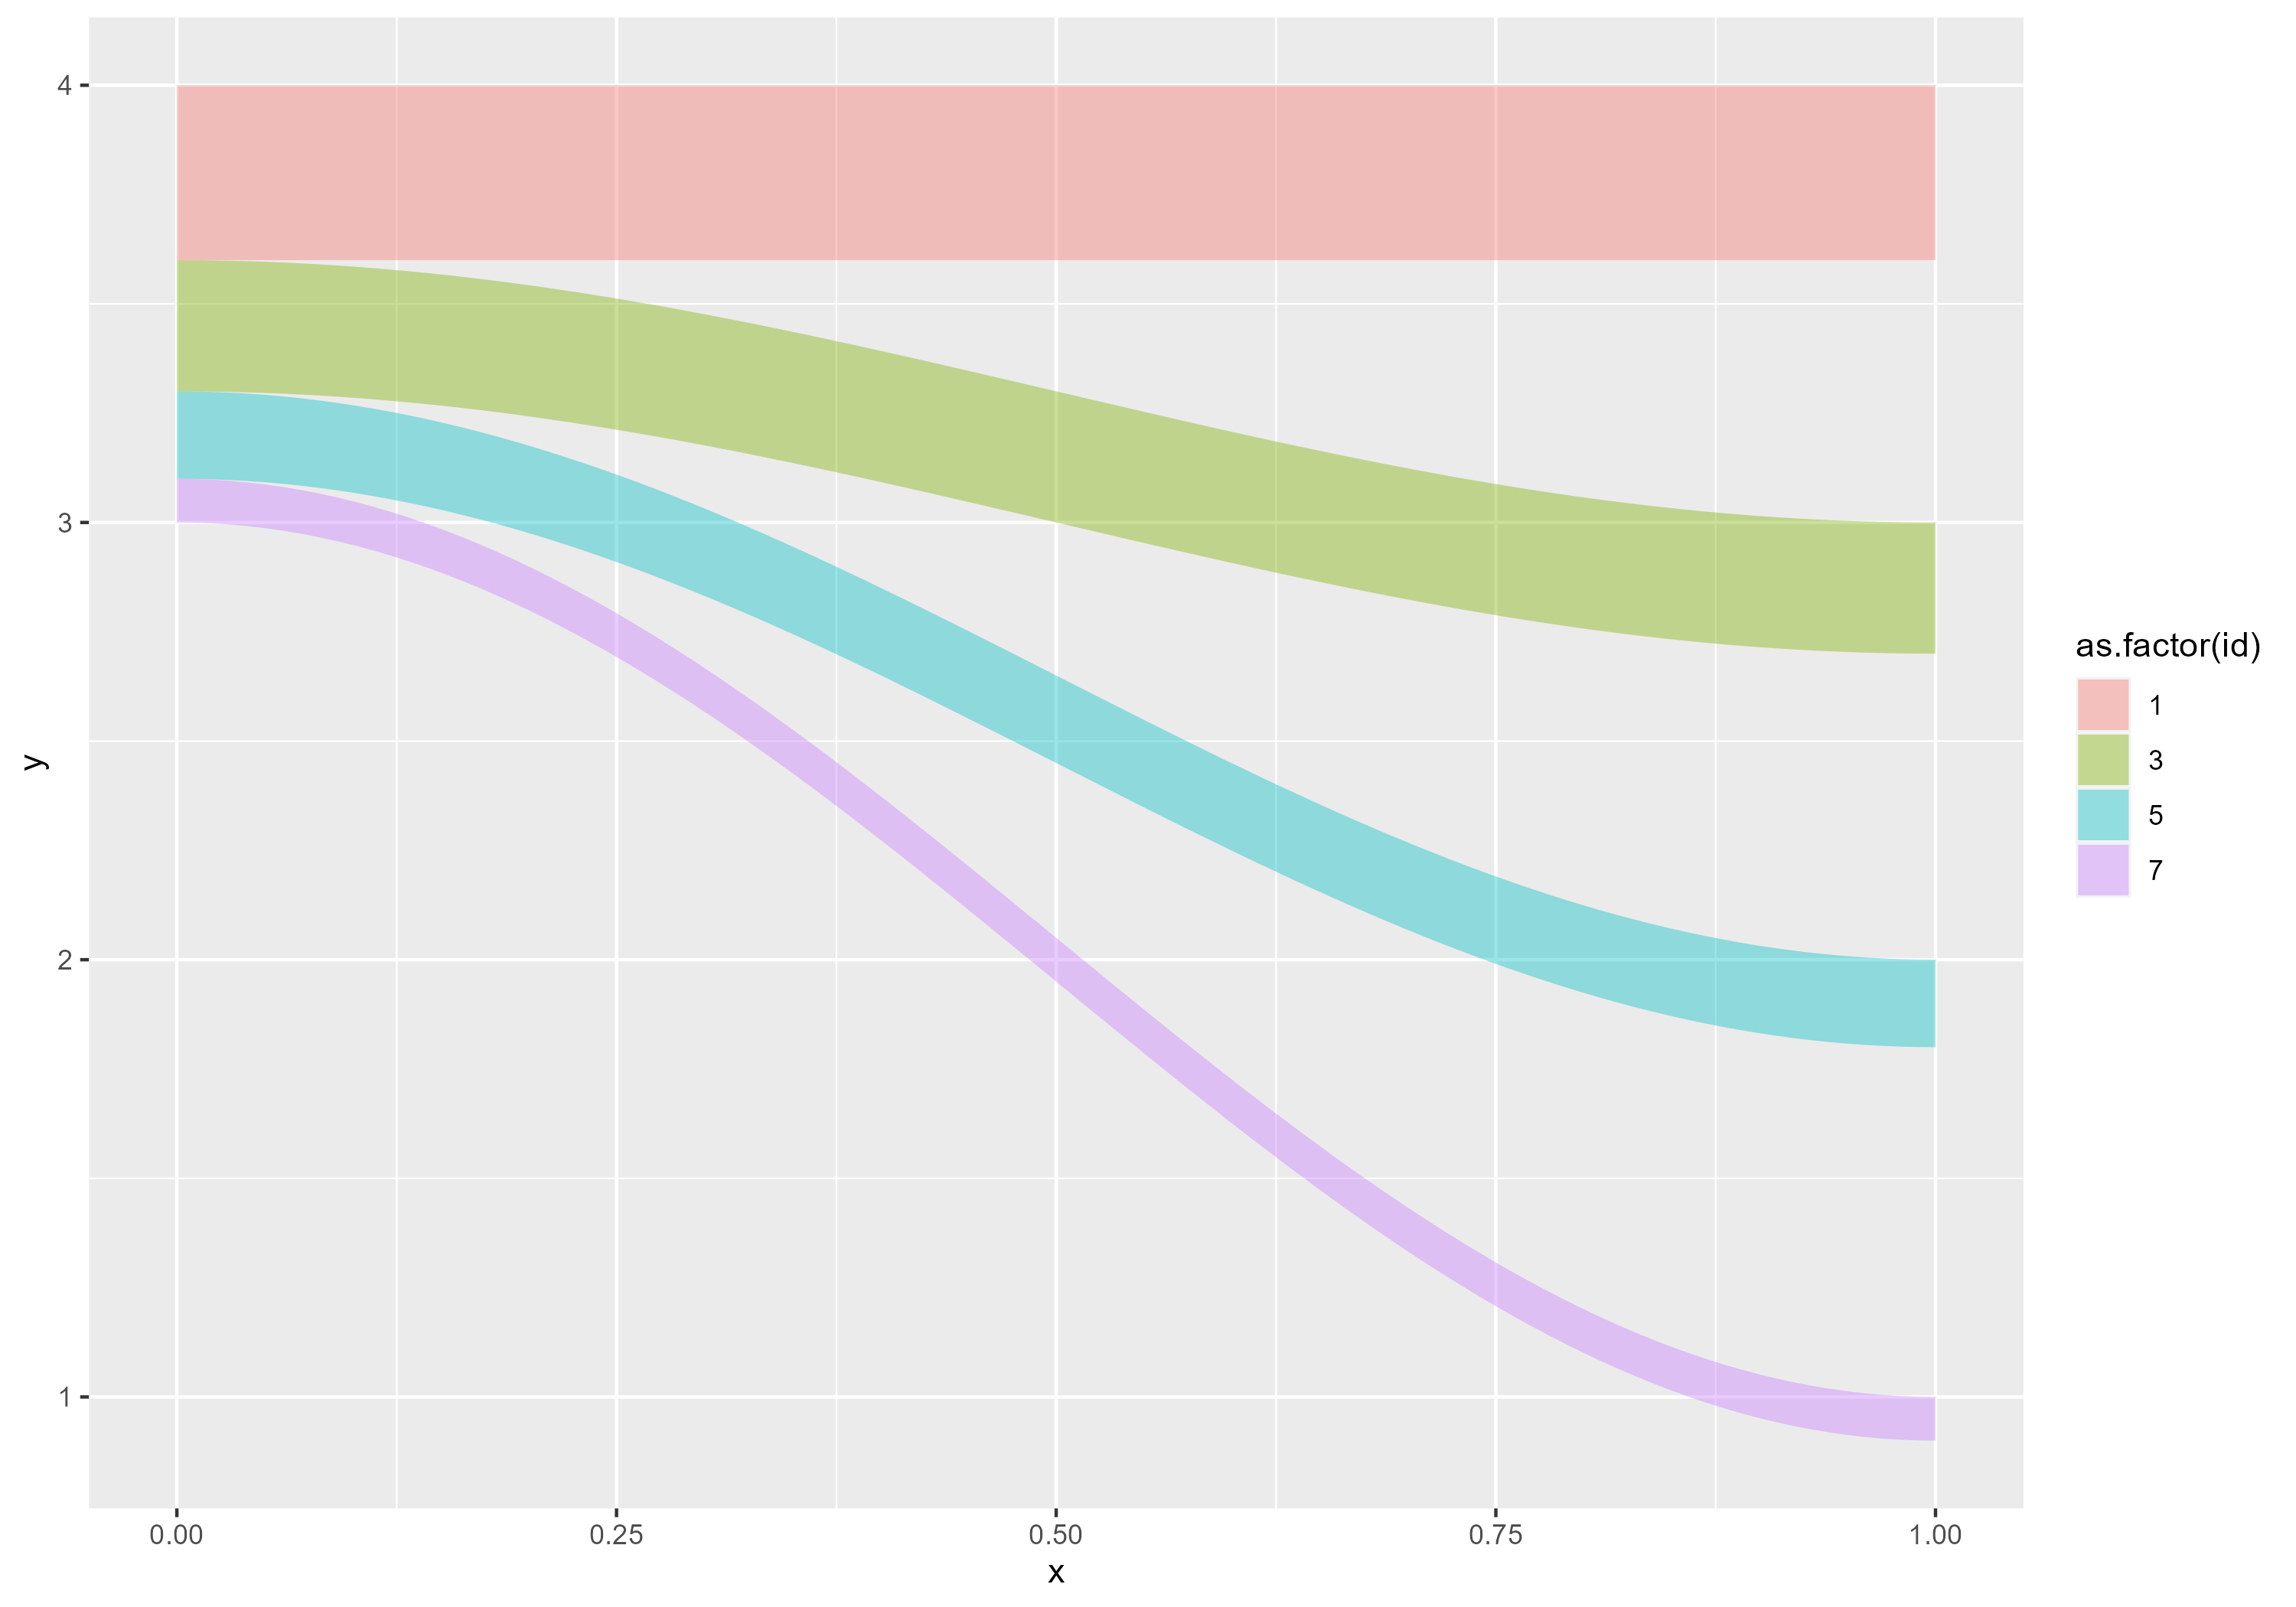
\includegraphics[width=0.5\linewidth]{figures/sine-shade} \caption{The plot shows the difference between the sigmoid (shown in the left figure) and the sine curve (shown in the right figure). In the sigmoid, as the curve progresses, it becomes narrower, resulting in a less accurate representation of proportions compared to the sine curve.}\label{fig:proportional-shade}
\end{figure}

In the animation, the proportional shaded area has been incorporated to facilitate a quick grasp of the proportion information. It displays the proportion of observation within each group. The design also needs to account for situations where the visualization lacks an adequate number of data points. In such cases, it can be challenging to visually discern the movement pattern of the subgroup, requiring the implementation of observation interpolation.

As mentioned in the Animation tools section, the paths of observations are getting interpolated. These functions only generate a linear path between points. However, linear paths may not be suitable for creating proportional shading, as they do not accurately represent the proportions. Non-linear curves like the sigmoid curves should be considered instead, as they provide a better display of proportions. These curves are commonly used in multiple Sankey diagrams, but there is a limitation on this shape. The issue is shown in Figure \ref{fig:proportional-shade}. While it does accurately represent the proportion at the beginning and end, as it curves, the shape gets narrower, leading to less accurate proportion representation (Shaffer (2019))

\hypertarget{software}{%
\section{Software}\label{software}}

\hypertarget{installation}{%
\subsection{Installation}\label{installation}}

The development version of \pkg{animbook} can be installed from \href{https://github.com/KrisanatA/animbook}{GitHub} with:

\begin{verbatim}
# install.packages("devtools")
devtools::install_github("KrisanatA/animbook")
\end{verbatim}

\hypertarget{overview-of-functions}{%
\subsection{Overview of functions}\label{overview-of-functions}}

In designing the \pkg{animbook} package, a three-step structured approach was developed to create an animation. The initial step is to reformat the data to the animated data structure as seen in \ref{fig:data-diagram}. The second stage is creating a \texttt{ggplot} object, which can be subsequently passed into the animation function. The final step involves transforming the \texttt{ggplot} to a \texttt{gganimate} object by integrating the animation settings. This three-step structure was implemented to ensure that users, regardless of their level of experience, can produce the animations with simplicity while retaining customization for more experienced users.

\hypertarget{data-preprocessing}{%
\subsubsection{Data preprocessing}\label{data-preprocessing}}

From Figure \ref{fig:data-diagram}, there is a need to map numerical value to a category. One way to handle this is by ranking the sales and grouping the rankings into quantiles. In some cases, this may not be the best option. When the observation is moved up by quantile, one is bound to move down. This issue can be resolved by using an alternative method, which is grouping values based on their absolute values. Users may also be interested in grouping the data based on different groups, for example, ranking within a specific country. This generalization leads to four different scaling methods for the numerical data.

\begin{verbatim}
#> # A tibble: 12 x 8
#>    id     time gp    values  rank rank_group absolute absolute_group
#>    <fct> <int> <fct>  <dbl> <int>      <int>    <int>          <int>
#>  1 1      2020 X      4255.     3          3        3              3
#>  2 1      2023 X      3357.     2          2        4              4
#>  3 14     2020 X      6763.     2          2        2              2
#>  4 14     2023 X      1197.     4          5        5              5
#>  5 100    2020 X      6864.     2          2        2              2
#>  6 100    2023 X      2321.     3          3        4              4
#>  7 21     2020 Y       698.     5          5        5              5
#>  8 21     2023 Y      3970.     2          2        4              3
#>  9 106    2020 Y      4110.     3          3        3              3
#> 10 106    2023 Y      2866.     3          3        4              4
#> 11 148    2020 Y      7174.     2          2        2              2
#> 12 148    2023 Y      4217.     1          1        3              3
\end{verbatim}

\begin{enumerate}
\def\labelenumi{\arabic{enumi}.}
\tightlist
\item
  Ranking by year. (rank)
\item
  Ranking by year within a group. (rank\_group)
\item
  Fix bins relative to absolute values by year. (absolute)
\item
  Fix bins relative to absolute values by year within a group. (absolute\_group)
\end{enumerate}

For the first and second scaling methods, group splitting is executed using the \texttt{quantiles()} and \texttt{cut()} functions. The \texttt{quantile()} function from the \CRANpkg{stats} package (R Core Team (2013)) takes a numeric vector and outputs the corresponding quantiles to the given probabilities. The output from the \texttt{quantile()} function is then used as the \texttt{breaks} argument for the \texttt{cut()} function that is part of the base R packages (R Core Team (2021)).

In contrast, the third and fourth scaling methods calculate the quantile based on the absolute values scales. To avoid varying values scales among groups, the variables are first normalized to a range between 0 and 1. The default approach then breaks the group equally using the \texttt{seq()} function. The \texttt{seq()} function takes input values from 0 to 1 and increments by equal steps depending on the number of groups of interest. Additionally, the users have the option to specify the breaks themselves if they choose to do so.

These are only the initial steps in formatting the data into a category. Now that there is a method to transform the data from the raw into a categorized format, the next step is to modify it into an animated data structure. It is carried out by assigning the frame to each individual observation, ensuring that each ID does not contain repeat frame values. It lets the \CRANpkg{gganimate} or \CRANpkg{plotly} perceive where the observation would be on the plot at a given frame, as seen in Figure \ref{fig:animated-diagram}.

The frame variable is assigned by sorting the data based on the ID and time using the \texttt{arrange()} function, followed by applying the \texttt{group\_by()} function on the ID, allowing the \texttt{row\_number()} function to be performed within each group. The functions mentioned in this paragraph are from the \CRANpkg{dplyr} package (Wickham et al. (2023)).

All of the pre-processing steps mentioned above are completed using the \texttt{anim\_prep()} or \texttt{anim\_prep\_cat()} function, depending on the stages of the data structure. The \texttt{anim\_prep()} function is used for raw data format, while the \texttt{anim\_prep\_cat()} function is for categorized data format. There are additional arguments that allow users for more customization.

\begin{table}

\caption{\label{tab:tbl-required}The required argument for the prep function.}
\centering
\begin{tabular}[t]{l|l}
\hline
Argument & Description\\
\hline
data & A data frame containing the data to be prepared for visualization.\\
\hline
id & The column name that represents the unique identifier variable.\\
\hline
values & The column name that contains the numeric values to be visualized.\\
\hline
time & The column name represents the time variable.\\
\hline
\end{tabular}
\end{table}

\begin{table}

\caption{\label{tab:tbl-animprep}The argument in the anim\_prep for customized the data scaling.}
\centering
\begin{tabular}[t]{l|l}
\hline
Argument & Description\\
\hline
ngroup & The number of groups or categories to create for scaling values.\\
\hline
breaks & A vector of breaks for creating bins.\\
\hline
group\_scaling & The column name that represents the grouping variable.\\
\hline
\end{tabular}
\end{table}

\begin{table}

\caption{\label{tab:tbl-animprepcat}The argument in the anim\_prep\_cat for customized the order of the category.}
\centering
\begin{tabular}[t]{l|l}
\hline
Argument & Description\\
\hline
order & A vector of order for sorting the category values.\\
\hline
\end{tabular}
\end{table}

\begin{table}

\caption{\label{tab:tbl-visual}The additional argument for customizing the aesthetics of the visualization.}
\centering
\begin{tabular}[t]{l|l}
\hline
Argument & Description\\
\hline
label & A vector of labels to be used for the y-axis in the visualization.\\
\hline
color & The column name to be used in ggplot2::aes() for the plot function.\\
\hline
time\_dependent & Logical. Should the visualization be time-dependent? Default is TRUE.\\
\hline
runif\_min & The minimum value for random addition to frame numbers.\\
\hline
runif\_max & The maximum value for random addition to frame numbers.\\
\hline
\end{tabular}
\end{table}

In the \texttt{anim\_prep()} and \texttt{anim\_prep\_cat()}, there are required arguments that need to be specified. The lists are in the Table \ref{tab:tbl-required}.

As shown previously, there are a total of four different scaling for the \texttt{anim\_prep()} function. Both the use can customization of these scaling can be set using the following arguments in Table \ref{tab:tbl-animprep}.

For the \texttt{anim\_prep\_cat()} function, the arguments that allowed the user to order the category are by using this argument in Table \ref{tab:tbl-animprepcat}.

Then, for further customization regarding how the final visualization looks. The following arguments in Table \ref{tab:tbl-visual} can be adjusted.

\hypertarget{plotting-function}{%
\subsubsection{Plotting function}\label{plotting-function}}

Once the data is prepared. The next step is to create the \texttt{ggplot} object as a basis for the animation. There are three plots available in this package. Two of the plots could be used for the animation, and another plot is used as a static visualization. All of the plots have an internal function that converts the standard data format into the required structure for each plotting function.

\begin{itemize}
\tightlist
\item
  \texttt{kangaroo\_plot()}: plots the observation's movement over time.
\item
  \texttt{wallaby\_plot()}: the subset plot of the \texttt{kangaroo\_plot} with the time limit to only start and end.
\item
  \texttt{funnel\_web\_plot()}: the faceted static plot by time variable.
\end{itemize}

The main focus of this paper will be on the \texttt{wallaby\_plot()}, which draws inspiration from the New York Times animation and combines the knowledge gained from the previous sections in creating the visualization.

The \texttt{wallaby\_data()} function is responsible for performing data manipulation and formatting tasks on the original object. It includes creating additional data components for labeling and shading. This function also responds by interpolating the non-linear path. It performs this task by mapping the \texttt{sine()} function provided in this package to each observation using the \texttt{map()} function from the \CRANpkg{purrr} package (Wickham and Henry (2023)). The frame is recalculated using the same method mentioned in the data preprocessing section. The \texttt{sankey\_shade()} function is called to generate the proportional shaded data.

\begin{figure}
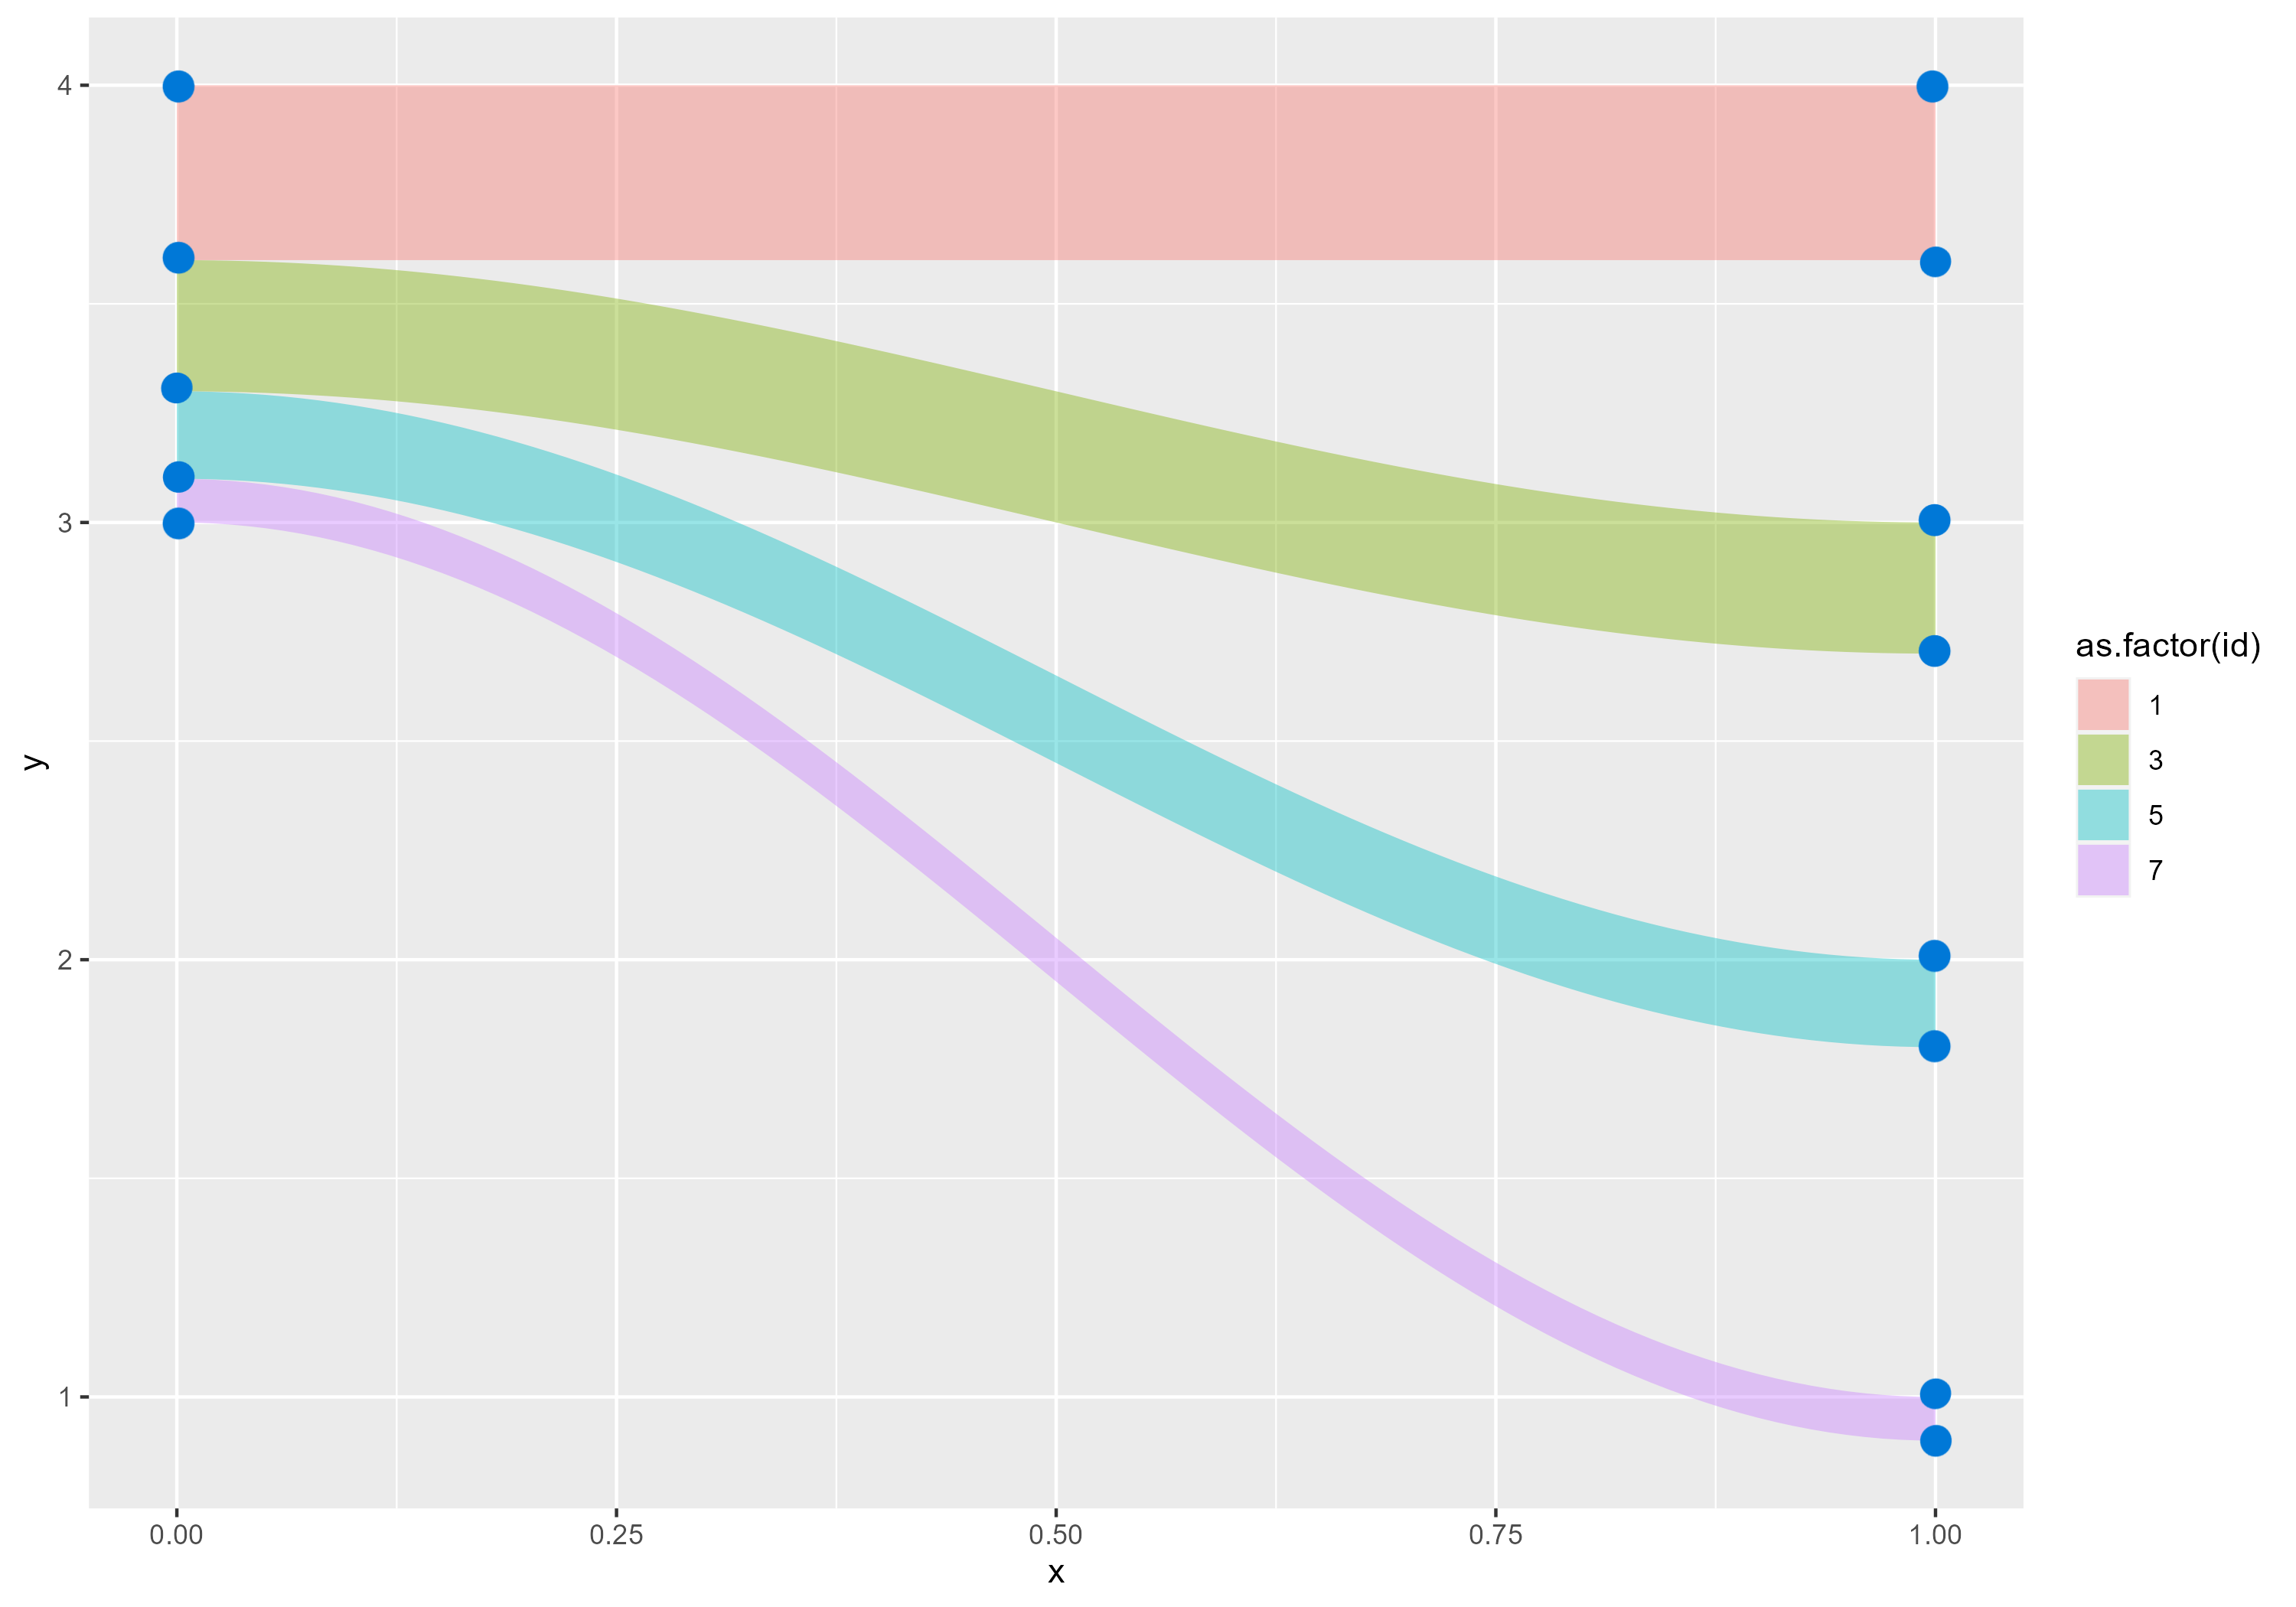
\includegraphics[width=0.5\linewidth]{figures/sankey-shade-1} 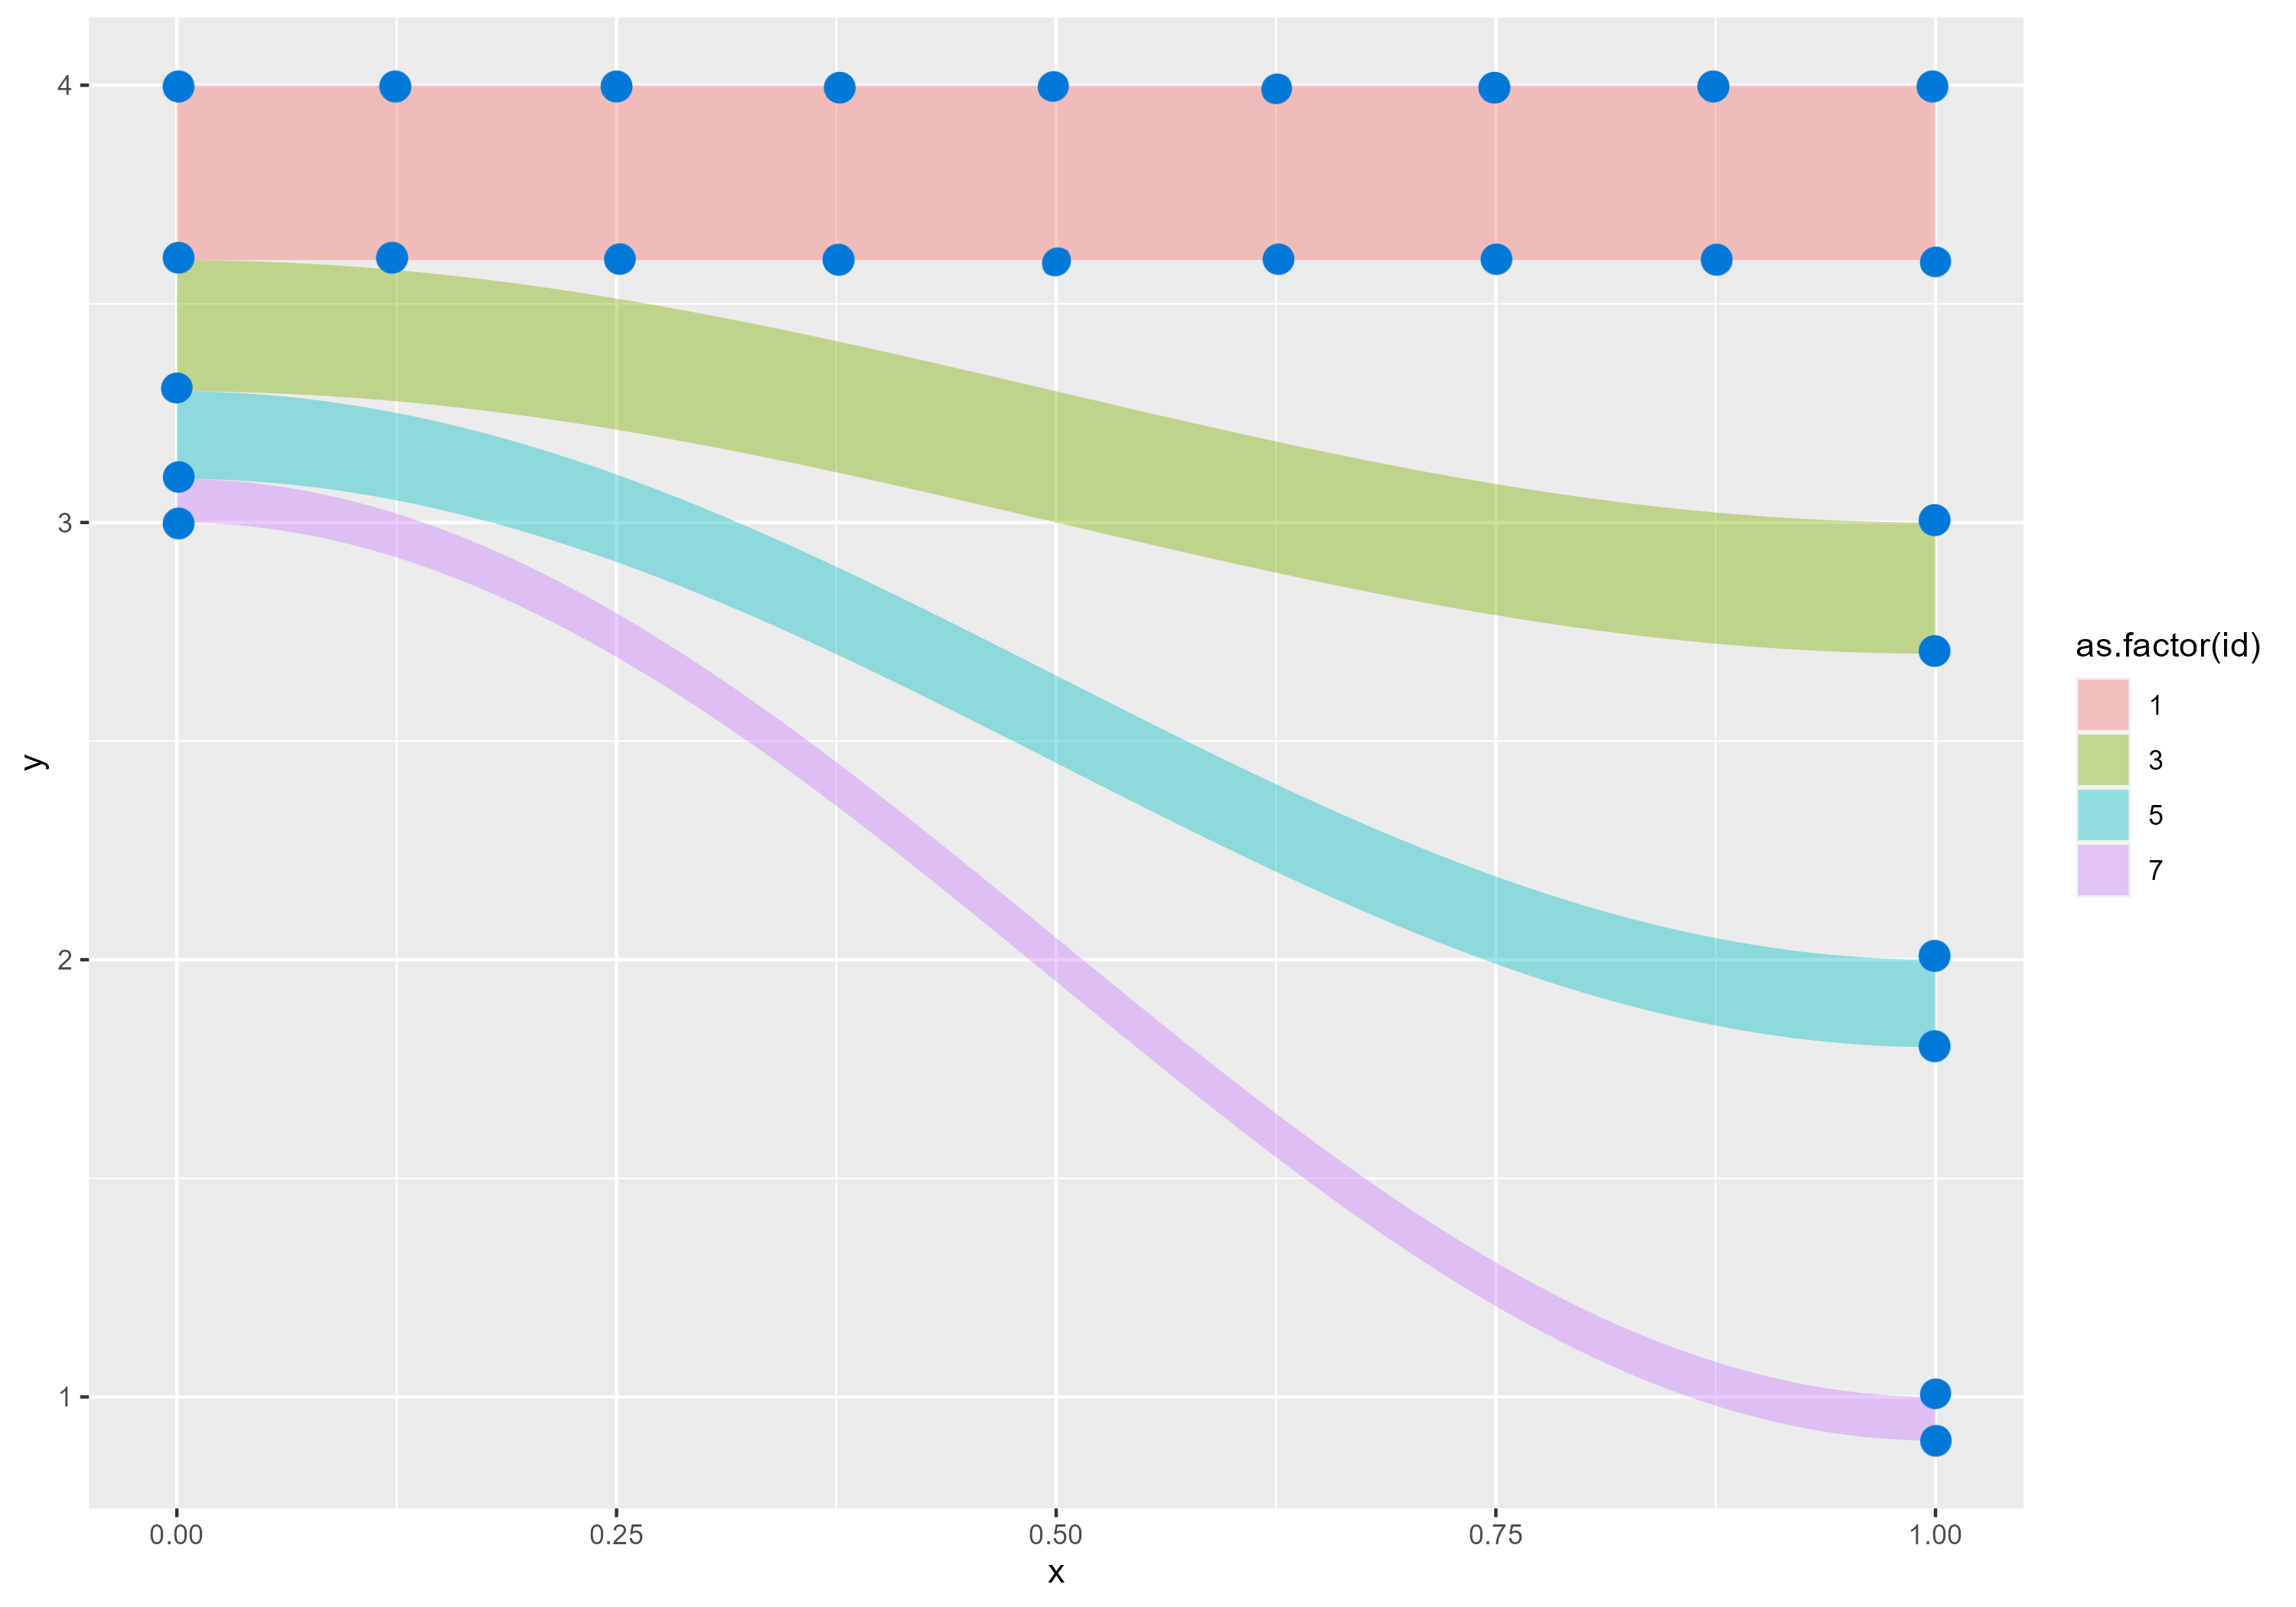
\includegraphics[width=0.5\linewidth]{figures/sankey-shade-2} \caption{The plot shows how the algorithm for the sankey\_shade() function works. The left figure represents the initial step of the algorithm, which calculates all the corner points. The right figure demonstrates the subsequent step, where points in-between the left and right are interpolated using the sine() function.}\label{fig:shade-algorithm}
\end{figure}

The algorithm behind the \texttt{sankey\_shade()} function for generating the proportional shaded data is illustrated in Figure \ref{fig:shade-algorithm}. It started by calculating the corner points for all of the shaded areas. Then, use the \texttt{sine()} function to interpolate the point between the left and right.

Now that the data are in the right format for the wallaby's plot, the \texttt{geom\_point()} function is used for plotting the observations, \texttt{geom\_polygon()} is used for creating the proportional shaded areas, and \texttt{geom\_text()} is used for creating labels. These three functions are from the \CRANpkg{ggplot2} package. During this process, the aesthetics mapping will be different depending on the rendering tool to be used, which can be either \texttt{gganimate} or \texttt{plotly}. The difference between the two rendering tools is that for \texttt{plotly}, the \texttt{ids} and \texttt{frame} arguments need to be specified during the creation of the \texttt{ggplot} object.

\begin{table}

\caption{\label{tab:unnamed-chunk-8}The arguments for the wallaby\_plot function.}
\centering
\begin{tabular}[t]{l|>{\raggedright\arraybackslash}p{30em}}
\hline
Argument & Description\\
\hline
object & The animbook object returned from the prep function.\\
\hline
group\_palette & The vector of the palette used by the function to supply the color to each group.\\
\hline
shade\_palette & The vector of the palette used by the function to supply the color to the shaded area.\\
\hline
rendering & The choice of method used to create and display the plot, either gganimate or plotly.\\
\hline
subset & A character string specifying the variable used for subsetting the data. The "top" and "bottom" strings can also be used in this argument.\\
\hline
relation & The choice of relationship for the values to display on the plot, either "one\_many." or "many\_one."\\
\hline
total\_point & The number of points the users want for the wallaby plot. Default is NULL, which is the number of points equal to the original.\\
\hline
height & The proportion of the area occupied by the observations in the shaded areas.\\
\hline
width & The distance between the first and last observation in the animation.\\
\hline
size & The point size.\\
\hline
alpha & The opacity of the proportional shaded areas.\\
\hline
\end{tabular}
\end{table}

\hypertarget{animating-function}{%
\subsubsection{Animating function}\label{animating-function}}

It is necessary to save the plot as a \texttt{ggplot} object before passing it to the final function, \texttt{anim\_animate()}, to animate. This function will automatically detect which rendering method was specified in the previous steps and add the minimum requirement functions accordingly. By default, if the user specifies the rendering as \texttt{gganimate}, then it will add the \texttt{transition\_time()} function from the \CRANpkg{gganimate} package. Otherwise, the \texttt{animation\_opts()} function will be added from the \CRANpkg{plotly} package.

\hypertarget{example-usage}{%
\subsection{Example usage}\label{example-usage}}

In this section, the package usage will be demonstrated using the \texttt{cat\_change} dataset included in this package. This dataset is simulated data that has changed from category A to E between two time points. Since this data is already in the categorized data structure, the \texttt{anim\_prep\_cat()} function is utilized.

The output produced from this package is referred to as the \texttt{animbook} object. This contained a list of data and settings that hold prepared data for visualization, along with a list of settings used in the plot function.

\begin{verbatim}
animbook <- anim_prep_cat(cat_change, 
                          id = id, 
                          values = qnt, 
                          time = time, 
                          color = gp, 
                          time_dependent = FALSE)

head(animbook$data, 10)
\end{verbatim}

\begin{verbatim}
#> # A tibble: 10 x 5
#>    id     time qtile frame color
#>    <fct> <int> <dbl> <dbl> <fct>
#>  1 1      2020     5    33 X    
#>  2 1      2023     5    34 X    
#>  3 2      2020     5     5 X    
#>  4 2      2023     5     6 X    
#>  5 3      2020     5    48 X    
#>  6 3      2023     5    49 X    
#>  7 4      2020     5    33 X    
#>  8 4      2023     5    34 X    
#>  9 5      2020     5     3 X    
#> 10 5      2023     5     4 X
\end{verbatim}

\begin{verbatim}
str(animbook)
\end{verbatim}

\begin{verbatim}
#> List of 2
#>  $ data    : tibble [400 x 5] (S3: tbl_df/tbl/data.frame)
#>   ..$ id   : Factor w/ 200 levels "1","2","3","4",..: 1 1 2 2 3 3 4 4 5 5 ...
#>   ..$ time : int [1:400] 2020 2023 2020 2023 2020 2023 2020 2023 2020 2023 ...
#>   ..$ qtile: num [1:400] 5 5 5 5 5 5 5 5 5 5 ...
#>   ..$ frame: num [1:400] 33 34 5 6 48 49 33 34 3 4 ...
#>   ..$ color: Factor w/ 2 levels "X","Y": 1 1 1 1 1 1 1 1 1 1 ...
#>  $ settings:List of 7
#>   ..$ gap           : num 0.1
#>   ..$ xbreaks       : int [1:2] 2020 2023
#>   ..$ label         : chr [1:5] "A" "B" "C" "D" ...
#>   ..$ order         : chr [1:5] "A" "B" "C" "D" ...
#>   ..$ time_dependent: logi FALSE
#>   ..$ runif_min     : num 1
#>   ..$ runif_max     : num 50
#>  - attr(*, "class")= chr "animbook"
\end{verbatim}

To obtain a \texttt{ggplot} object for the animation function, the \texttt{wallaby\_plot} is used. For further customization, the \texttt{shade\_palette}, \texttt{subset}, and \texttt{relation} arguments are applied to define the final appearance of the animation.

\begin{verbatim}
p <- wallaby_plot(object = animbook,
             group_palette = RColorBrewer::brewer.pal(9, "Set1"),
             shade_palette = c("#737373", "#969696", "#BDBDBD",
                               "#D9D9D9","#D9D9D9","#D9D9D9"),
             rendering = "ggplot",
             subset = "top",
             relation = "one_many",
             total_point = NULL)

p
\end{verbatim}

\begin{center}\includegraphics[width=1\linewidth]{animbook-journal_files/figure-latex/unnamed-chunk-10-1} \end{center}

Once the \texttt{ggplot} object is obtained, the \texttt{anim\_animate()} function can be used to transform it into a \texttt{gganimate} object. This then can be passed onto the \texttt{animate()} function from the \CRANpkg{gganimate} for rendering.

\begin{verbatim}
p2 <- anim_animate(p)

gganimate::animate(p2)
\end{verbatim}

\begin{figure}

{\centering 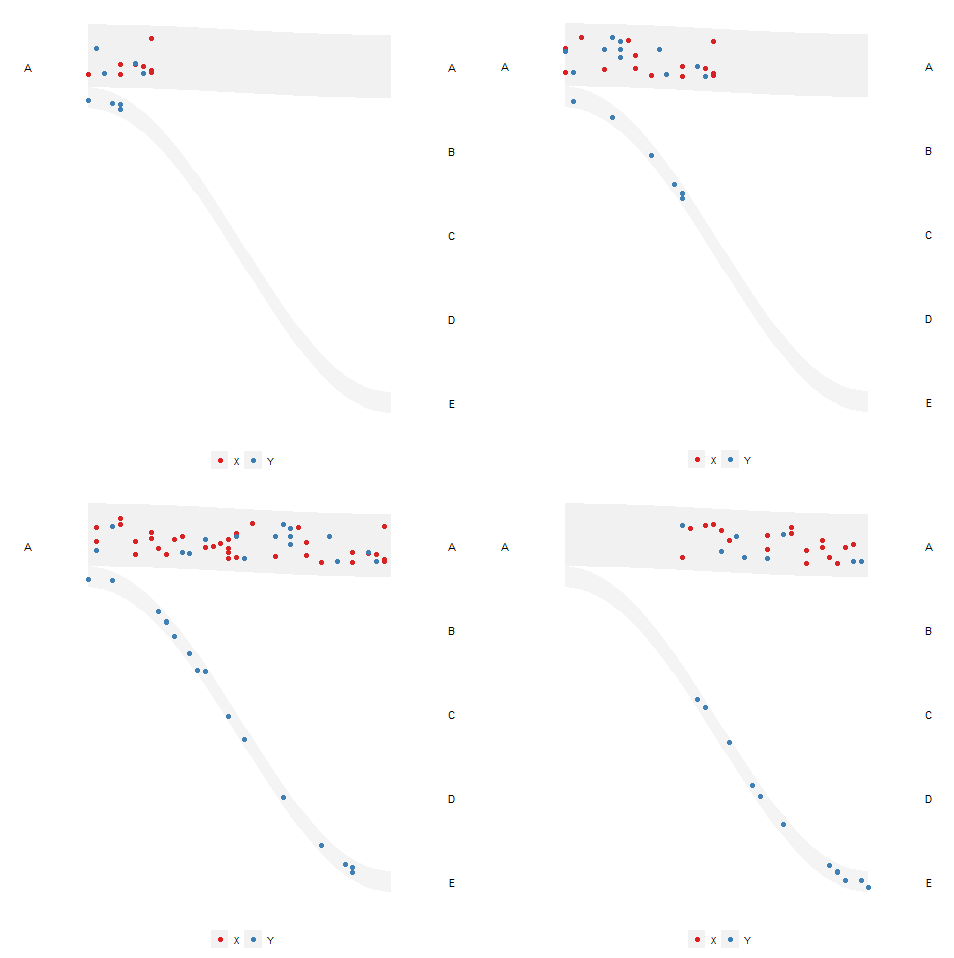
\includegraphics[width=1\linewidth]{figures/animation-example} 

}

\caption{Animate visualization using example data. All of the X observations stay within the same group, while Y observations change from group A to group E.}\label{fig:catchange-figure}
\end{figure}

This is an example of how the users can apply the three-step process in creating an animation plot using the \texttt{animbook} package.

\hypertarget{application}{%
\section{Application}\label{application}}

\hypertarget{accounting-database-osiris}{%
\subsection{Accounting database: osiris}\label{accounting-database-osiris}}

The accounting Osiris data that will be used in this section was collected from Bureau van Dijk ({``Osiris''} (n.d.)). This data set comprises 30,000 rows and 94 variables of information on listed and major unlisted/delisted companies worldwide. The only variables of interest from this data set are ID, year, country, and sales. A subset version of this data set, which only contained variables of interest from 2006 to 2018, is included in this package.

As mentioned in the OECD report (McGowan, Andrews, and Millot (2017)), the United States has a faster metabolize rate relative to Japan company. An animation will be created using the \texttt{animbook} package to enhance communication with data. First, filter the countries to include only the United States and Japan. Then, prepare the Osiris data using the \texttt{anim\_prep} function with the first scaling, which is a ranking method. Next, use the \texttt{wallaby\_plot} function to create a \texttt{ggplot} object and add default settings for \texttt{gganimate} rendering.

\begin{verbatim}
# library(animbook)
# library(dplyr)

data <- osiris |> 
  filter(country %in% c("US", "JP"))

label <- c("Top 25%", "25-50", "50-75", "75-100", "Not listed")

accounting <- anim_prep(data, 
                      id = ID, 
                      values = sales, 
                      time = year, 
                      label = label, 
                      ngroup = 4, 
                      color = country, 
                      time_dependent = FALSE)

p <- wallaby_plot(accounting,
                  group_palette = RColorBrewer::brewer.pal(9, "Set1"),
                  shade_palette = c("#737373", "#969696", "#BDBDBD",
                                    "#D9D9D9","#D9D9D9","#D9D9D9"),
                  subset = "bottom",
                  relation = "many_one",
                  height = 1,
                  size = 2,
                  width = 100,
                  total_point = 1000)

kan_p <- kangaroo_plot(accounting)

p2 <- anim_animate(p)
kan_p2 <- anim_animate(kan_p)
\end{verbatim}

\begin{verbatim}
gganimate::animate(p2)

gganimate::animate(kan_p2)
\end{verbatim}

\begin{figure}

{\centering 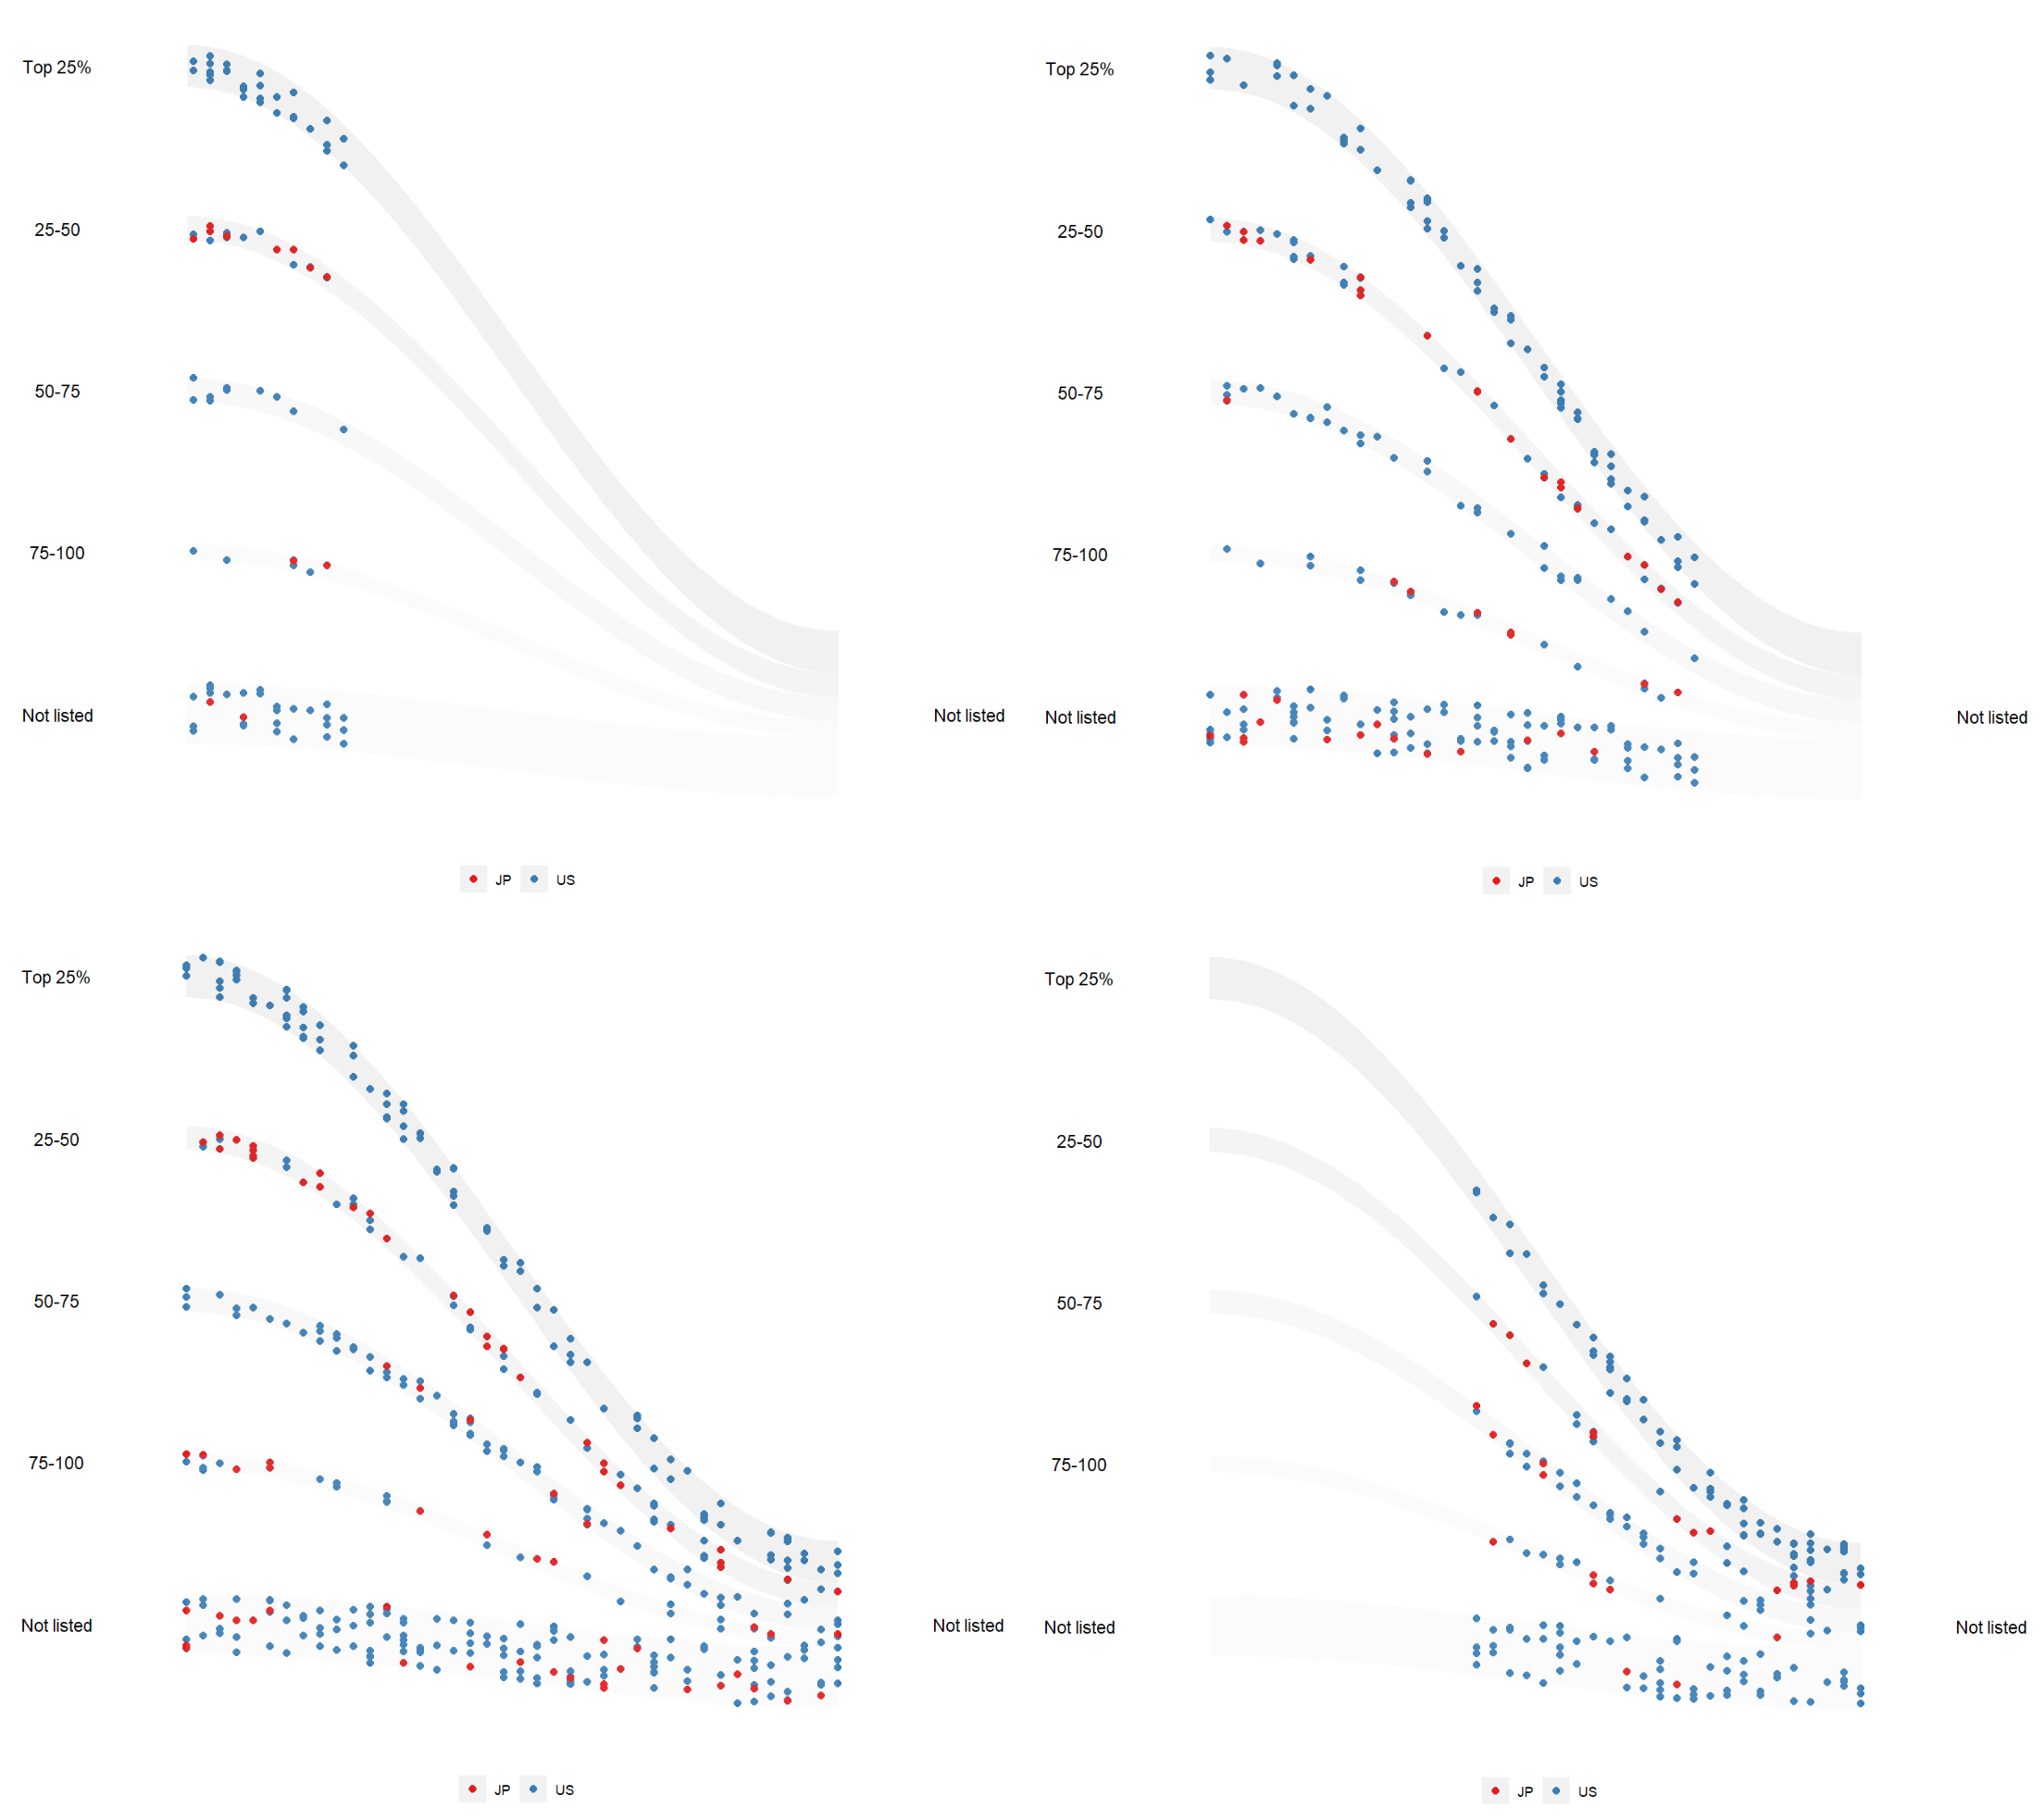
\includegraphics[width=1\linewidth]{figures/animation-exit} 

}

\caption{The animate visualization shows the companies that exited the market. There are more United States companies that fall down into a not listed group compared to Japanese companies.}\label{fig:osiris-figure}
\end{figure}

\begin{figure}

{\centering 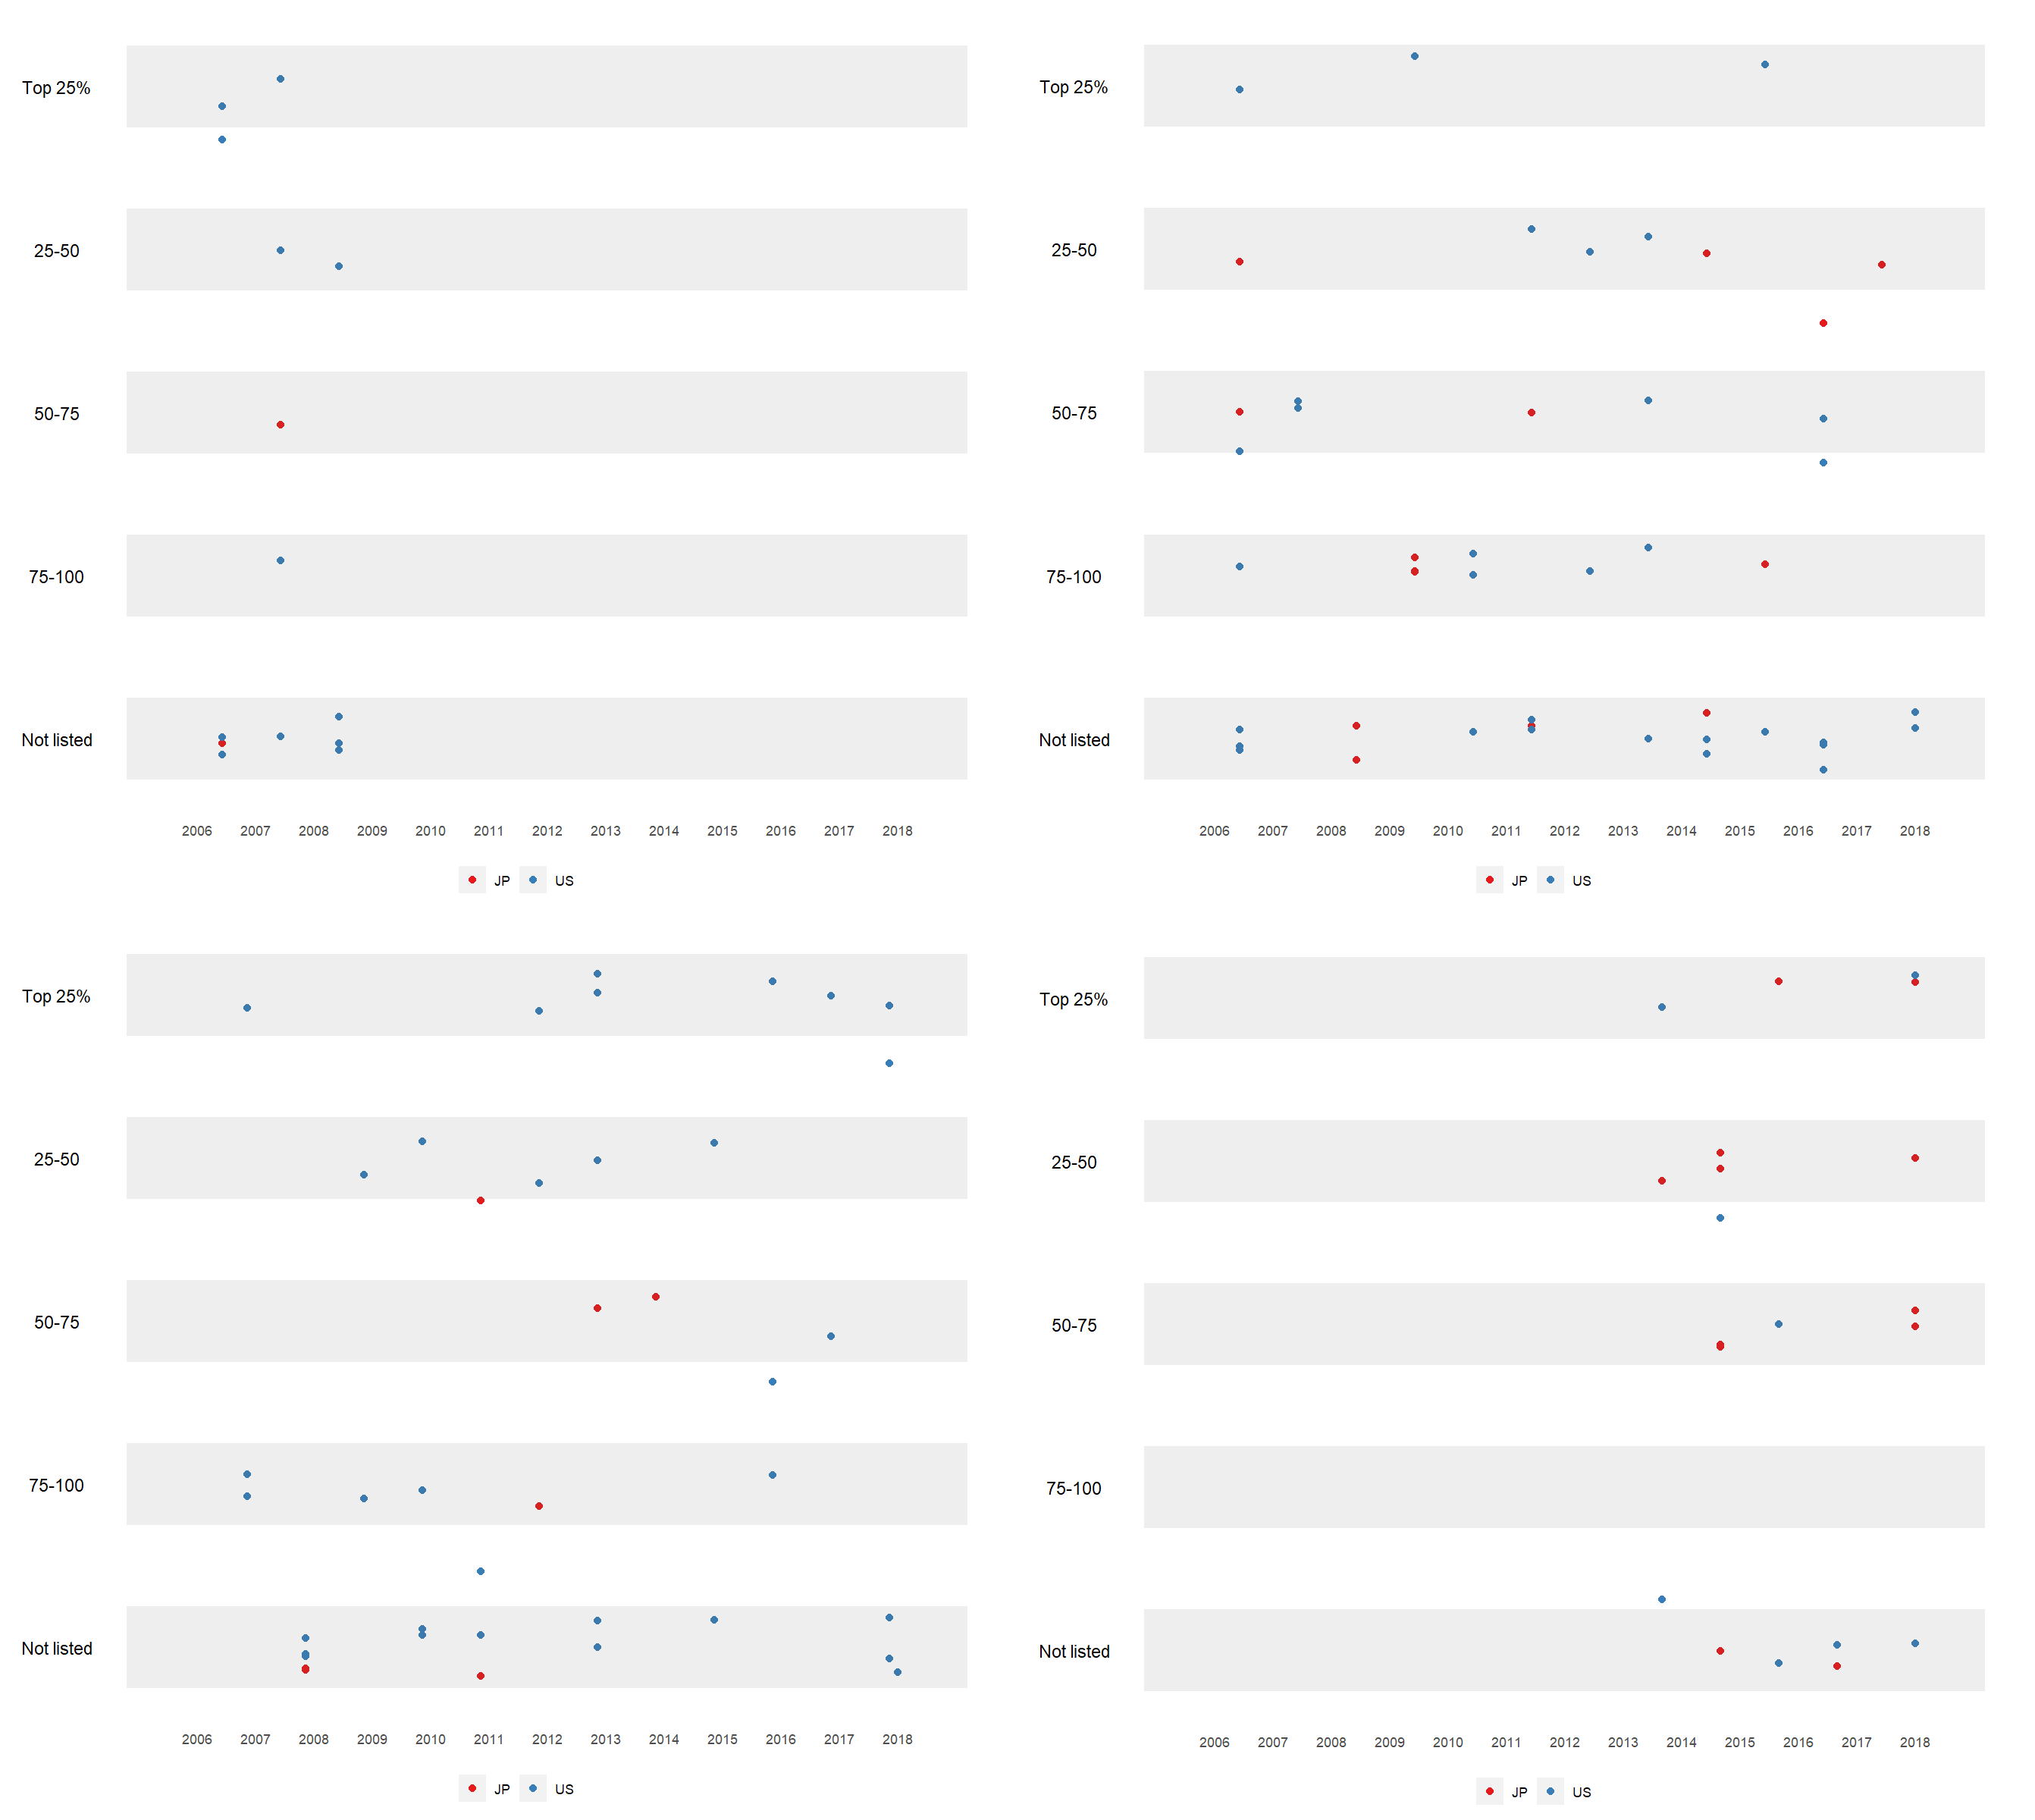
\includegraphics[width=1\linewidth]{figures/osiris} 

}

\caption{The animate visualization shows the movement of the companies between the groups from 2006 to 2018. In 2006, there were no Japanese companies in the Top 25\% group.}\label{fig:kan-osiris-figure}
\end{figure}

From the plot, a higher proportion of US companies have exited the market, confirming the OECD report (McGowan, Andrews, and Millot (2017)) that the United States has a higher turnover rate than Japan. An interesting finding is that all of the top 25\% of companies that exited the market are only from the United States. It may be due to the absence of Japanese companies in the Top 25\% in 2006, or it could be that Japanese companies who started in the Top 25\% in 2006 did not delist. Figure \ref{fig:kan-osiris-figure}, confirmed that there are non-Japanese companies that start at the Top 25\% in 2006.

\hypertarget{voter-behavior}{%
\subsection{Voter behavior}\label{voter-behavior}}

The Australian Election Study data was collected from ADA Dataverse (McAllister et al. (2023)). The dataset included in the \pkg{animbook} package contains 1,468 rows and 4 variables of information: ID, year, party, and gender. This dataset comprises survey responses from the 2019 election. The year column was transformed from the two different questions to answer the question, based on the 2016 Australian election results, how the top party performs in keeping the old voters for different genders.

\begin{verbatim}
voter <- anim_prep_cat(data = aeles,
                       id = id,
                       values = party,
                       time = year,
                       color = gender,
                       order = NULL,
                       time_dependent = FALSE)

p_voter <- wallaby_plot(object = voter,
                  group_palette = RColorBrewer::brewer.pal(9, "Set1"),
                  shade_palette = c("#737373", "#969696", "#BDBDBD",
                                    "#D9D9D9","#D9D9D9","#D9D9D9"),
                  rendering = "ggplot",
                  subset = "top",
                  relation = "one_many",
                  height = 1,
                  size = 2,
                  width = 100,
                  total_point = 1000)

p2_voter <- anim_animate(p_voter)
\end{verbatim}

\begin{verbatim}
gganimate::animate(p2_voter)
\end{verbatim}

\begin{figure}

{\centering 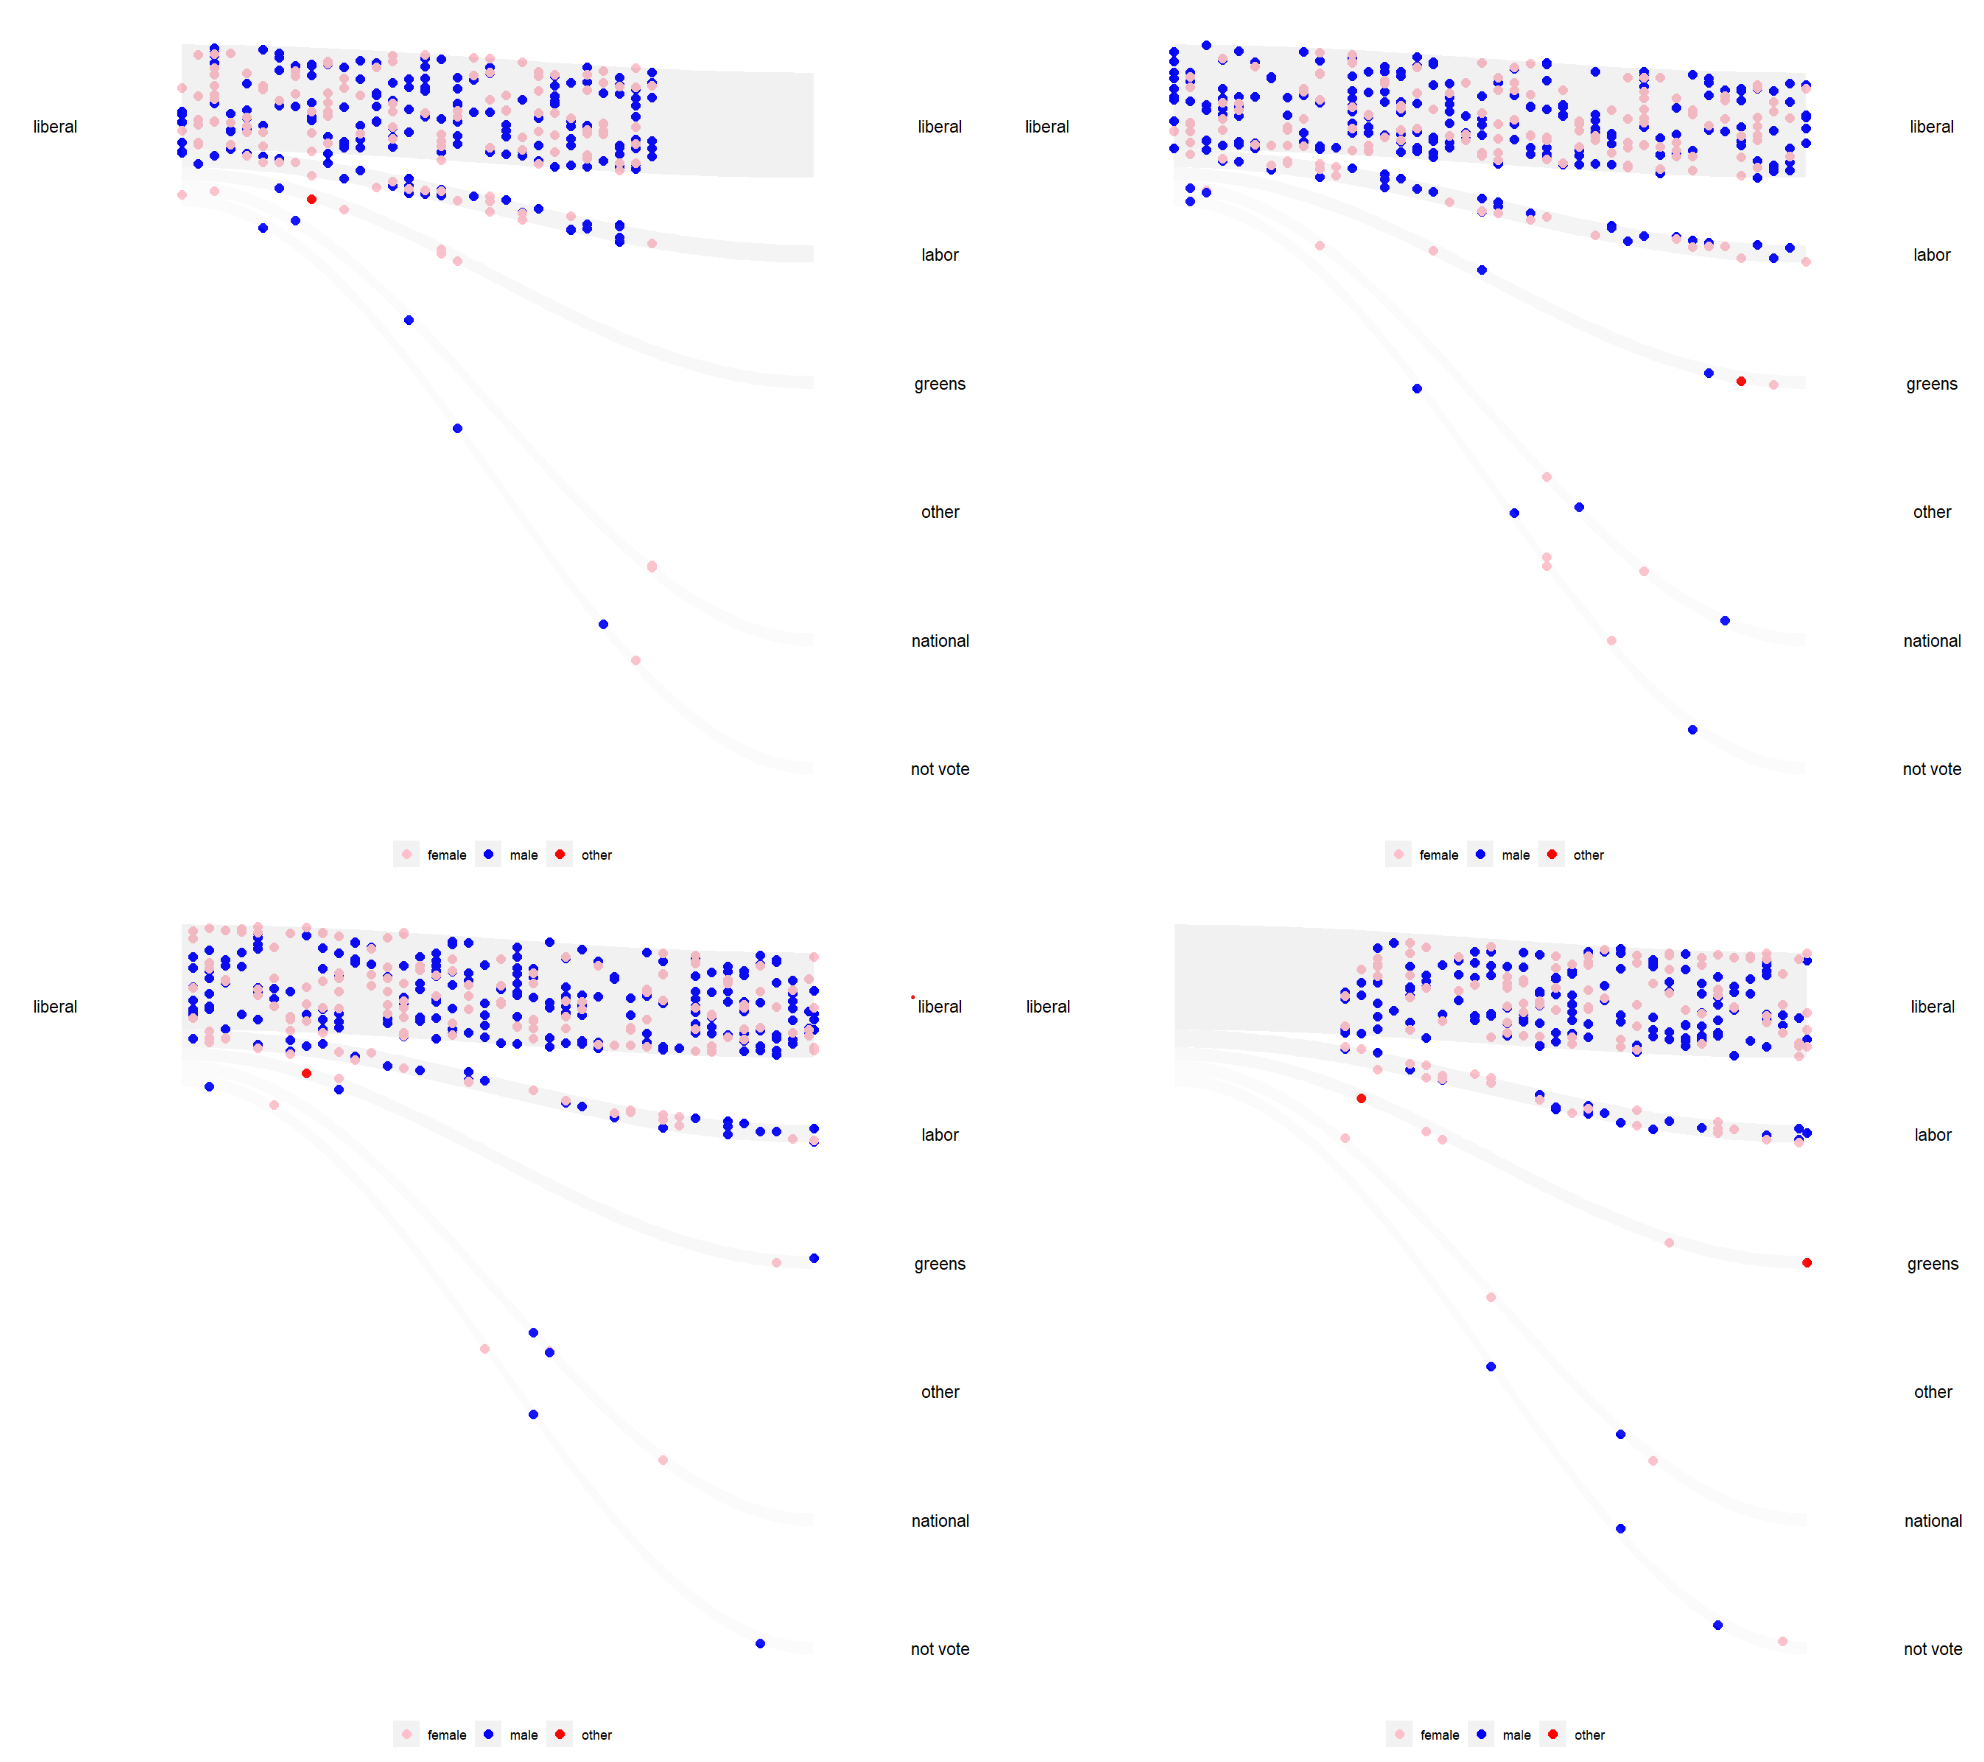
\includegraphics[width=1\linewidth]{figures/animation-voter} 

}

\caption{The animate visualization shows how does the top party perform in keeping the old voters for different genders. Most voters remain loyal to the party, but a small fraction of voters with roughly equal male-to-female ratio switch primarily to the other major party.}\label{fig:voter-figure}
\end{figure}

From Figure \ref{fig:voter-figure}, it is clear that individuals who identified their gender as `others' shifted their votes from the Liberal, the leading party in 2016, to the Greens party. These changes could be due to the Green Party's ``A FAIRER, MORE EQUAL COMMUNITY'' campaign, which advocates for full equality under the law and communities for LGBTIQ+ individuals. If the Liberal Party wishes to retain this demographic of voters, they may need to consider implementing a campaign focused on LGBTIQ+ issues.

\hypertarget{summary}{%
\section{Summary}\label{summary}}

Beginning with inspiration from the New York Times articles, this package provides tools to facilitate the communication of complex data to general audiences. In the current version of \pkg{animbook}, the feature to have different speeds for each observation has not yet been implemented. This feature will introduce a new dimension that allows the users to explore the data further. The plotly rendering is also not yet been optimized for use. Additionally, both new animated and static plots could also be added, as seen in the New York Times article (Badger et al. (2018)), to compare the demographics at a specific point in time. On top of that, the \CRANpkg{cli} package (Csárdi (2023)) could be used for a more aesthetically pleasing command-line interface.

\hypertarget{acknowledgements}{%
\section*{Acknowledgements}\label{acknowledgements}}
\addcontentsline{toc}{section}{Acknowledgements}

This paper is created using the \CRANpkg{rjtools} packages (O'Hara-Wild et al. (2023)) and is based on the 0.0.0.9 version of the \pkg{animbook} package. This version is available on \href{https://github.com/KrisanatA/animbook}{GitHub}.

I also acknowledge the use of ChatGPT (\url{https://chat.openai.com/}) to paraphrase the sentence.

\hypertarget{references}{%
\section*{References}\label{references}}
\addcontentsline{toc}{section}{References}

\hypertarget{refs}{}
\begin{CSLReferences}{1}{0}
\leavevmode\vadjust pre{\hypertarget{ref-the_new_york_time}{}}%
Badger, Emily, Claire Cain Miller, Adam Pearce, and Kevin Quealy. 2018. {``Extensive Data Shows Punishing Reach of Racism for Black Boys.''} \emph{The New York Times}. The New York Times. \url{https://www.nytimes.com/interactive/2018/03/19/upshot/race-class-white-and-black-men.html}.

\leavevmode\vadjust pre{\hypertarget{ref-d3js}{}}%
Bostock, Mike. 2012. {``D3.js - Data-Driven Documents.''} 2012. \url{http://d3js.org/}.

\leavevmode\vadjust pre{\hypertarget{ref-zombie_companies_2008}{}}%
Caballero, Ricardo J., Takeo Hoshi, and Anil K. Kashyap. 2008. {``Zombie Lending and Depressed Restructuring in {J}apan.''} \emph{The American Economic Review} 98 (5): 1943--77. \url{http://www.jstor.org/stable/29730158}.

\leavevmode\vadjust pre{\hypertarget{ref-race}{}}%
Chetty, Raj, Nathaniel Hendren, Maggie Jones, and Sonya Porter. 2020. {``Race and Economic Opportunity in the United States: An Intergenerational Perspective*.''} \emph{The Quarterly Journal of Economics} 135 (May): 711--83. \url{https://doi.org/10.1093/qje/qjz042}.

\leavevmode\vadjust pre{\hypertarget{ref-cli}{}}%
Csárdi, Gábor. 2023. \emph{Cli: Helpers for Developing Command Line Interfaces}. \url{https://CRAN.R-project.org/package=cli}.

\leavevmode\vadjust pre{\hypertarget{ref-learner-control}{}}%
Hasler, Béatrice, Bernd Kersten, and John Sweller. 2007. {``Learner Control, Cognitive Load and Instructional Animation. Applied Cognitive Psychology, 21, 713-729.''} \emph{Applied Cognitive Psychology} 21 (September): 713--29. \url{https://doi.org/10.1002/acp.1345}.

\leavevmode\vadjust pre{\hypertarget{ref-mayer-2010}{}}%
Mayer, Richard. 2010. {``Applying the Science of Learning to Medical Education.''} \emph{Medical Education} 44 (June): 543--49. \url{https://doi.org/10.1111/j.1365-2923.2010.03624.x}.

\leavevmode\vadjust pre{\hypertarget{ref-mayer_2005}{}}%
Mayer, Richard E. 2005. {``Cognitive Theory of Multimedia Learning.''} In \emph{The Cambridge Handbook of Multimedia Learning}, edited by RichardEditor Mayer, 31--48. Cambridge Handbooks in Psychology. Cambridge University Press. \url{https://doi.org/10.1017/CBO9780511816819.004}.

\leavevmode\vadjust pre{\hypertarget{ref-Mayer_Moreno_2002}{}}%
Mayer, Richard E., and Roxana Moreno. 2002. \emph{Educational Psychology Review} 14 (1): 87--99. \url{https://doi.org/10.1023/a:1013184611077}.

\leavevmode\vadjust pre{\hypertarget{ref-aeles}{}}%
McAllister, Ian, Jill Sheppard, Sarah Cameron, and Jackman Simon. 2023. {``Australian Election Study, 2022.''} ADA Dataverse. \url{https://doi.org/10.26193/W3U2S3}.

\leavevmode\vadjust pre{\hypertarget{ref-oecd_report}{}}%
McGowan, Müge Adalet, Dan Andrews, and Valentine Millot. 2017. {``The Walking Dead?''} no. 1372. https://doi.org/\url{https://doi.org/https://doi.org/10.1787/180d80ad-en}.

\leavevmode\vadjust pre{\hypertarget{ref-rjtools}{}}%
O'Hara-Wild, Mitchell, Stephanie Kobakian, H. Sherry Zhang, Di Cook, Simon Urbanek, and Christophe Dervieux. 2023. \emph{Rjtools: Preparing, Checking, and Submitting Articles to the 'r Journal'}. \url{https://CRAN.R-project.org/package=rjtools}.

\leavevmode\vadjust pre{\hypertarget{ref-av}{}}%
Ooms, Jeroen. 2023a. \emph{Av: Working with Audio and Video in r}. \url{https://CRAN.R-project.org/package=av}.

\leavevmode\vadjust pre{\hypertarget{ref-gifski}{}}%
---------. 2023b. \emph{Gifski: Highest Quality GIF Encoder}. \url{https://CRAN.R-project.org/package=gifski}.

\leavevmode\vadjust pre{\hypertarget{ref-bvd}{}}%
{``Osiris.''} n.d. \emph{Bvd}. Bureau van Dijk. \url{https://www.bvdinfo.com/en-gb/our-products/data/international/osiris}.

\leavevmode\vadjust pre{\hypertarget{ref-tweenr}{}}%
Pedersen, Thomas Lin. 2022. \emph{Tweenr: Interpolate Data for Smooth Animations}. \url{https://CRAN.R-project.org/package=tweenr}.

\leavevmode\vadjust pre{\hypertarget{ref-gganimate}{}}%
Pedersen, Thomas Lin, and David Robinson. 2020. {``Gganimate: A Grammar of Animated Graphics.''} \emph{R Package Version} 1 (7): 403--8.

\leavevmode\vadjust pre{\hypertarget{ref-stats}{}}%
R Core Team. 2013. \emph{R: A Language and Environment for Statistical Computing}. Vienna, Austria: R Foundation for Statistical Computing. \url{http://www.R-project.org/}.

\leavevmode\vadjust pre{\hypertarget{ref-r}{}}%
---------. 2021. \emph{R: A Language and Environment for Statistical Computing}. Vienna, Austria: R Foundation for Statistical Computing. \url{https://www.R-project.org/}.

\leavevmode\vadjust pre{\hypertarget{ref-effective-trend}{}}%
Robertson, George, Roland Fernandez, Danyel Fisher, Bongshin Lee, and John Stasko. 2008. {``Effectiveness of Animation in Trend Visualization.''} \emph{IEEE Transactions on Visualization and Computer Graphics} 14 (6): 1325--32. \url{https://doi.org/10.1109/TVCG.2008.125}.

\leavevmode\vadjust pre{\hypertarget{ref-Shaffer_2019}{}}%
Shaffer, Jeffrey. 2019. {``Sankey Diagrams: Why i Used the Sigmoid Function and Why You Probably Shouldn't.''} \emph{Data + Science}. \url{https://www.dataplusscience.com/Sigmoid.html}.

\leavevmode\vadjust pre{\hypertarget{ref-plotly}{}}%
Sievert, Carson. 2020. {``Interactive {Web-Based} Data Visualization with r, Plotly, and Shiny.''} Chapman; Hall/CRC. \url{https://plotly-r.com}.

\leavevmode\vadjust pre{\hypertarget{ref-animation-mechanic}{}}%
Webster, Chris. 2005. \emph{Animation : The Mechanics of Motion}. Focal Press Visual Effects and Animation Series. Oxford ; Burlington, MA: Elsevier Focal Press.

\leavevmode\vadjust pre{\hypertarget{ref-tidy-data}{}}%
Wickham, Hadley. 2014. {``Tidy Data.''} \emph{Journal of Statistical Software} 59 (10): 1--23. \url{https://doi.org/10.18637/jss.v059.i10}.

\leavevmode\vadjust pre{\hypertarget{ref-ggplot2}{}}%
---------. 2016. \emph{Ggplot2: Elegant Graphics for Data Analysis}. Springer-Verlag New York. \url{https://ggplot2.tidyverse.org}.

\leavevmode\vadjust pre{\hypertarget{ref-dplyr}{}}%
Wickham, Hadley, Romain François, Lionel Henry, Kirill Müller, and Davis Vaughan. 2023. \emph{Dplyr: A Grammar of Data Manipulation}.

\leavevmode\vadjust pre{\hypertarget{ref-purrr}{}}%
Wickham, Hadley, and Lionel Henry. 2023. \emph{Purrr: Functional Programming Tools}. \url{https://CRAN.R-project.org/package=purrr}.

\end{CSLReferences}

\bibliography{animbook-journal.bib}

\address{%
Krisanat Anukarnsakulchularp\\
Monash University\\%
Department of Econometrics and Business Statistics\\ Melbourne, Australia\\
%
%
\textit{ORCiD: \href{https://orcid.org/0009-0008-5638-7124}{0009-0008-5638-7124}}\\%
\href{mailto:kanu0003@student.monash.edu}{\nolinkurl{kanu0003@student.monash.edu}}%
}
